%% 
%% Copyright 2007-2020 Elsevier Ltd
%% 
%% This file is part of the 'Elsarticle Bundle'.
%% ---------------------------------------------
%% 
%% It may be distributed under the conditions of the LaTeX Project Public
%% License, either version 1.3 of this license or (at your option) any
%% later version.  The latest version of this license is in
%%    http://www.latex-project.org/lppl.txt
%% and version 1.3 or later is part of all distributions of LaTeX
%% version 1999/12/01 or later.
%% 
%% The list of all files belonging to the 'Elsarticle Bundle' is
%% given in the file `manifest.txt'.
%% 
%% Template article for Elsevier's document class `elsarticle'
%% with numbered style bibliographic references
%% SP 2008/03/01
%% $Id: elsarticle-template-num.tex 213 2021-11-17 03:42:37Z apu.v $
%%
%\documentclass[preprint,12pt]{elsarticle}

%% Use the option review to obtain double line spacing
%% \documentclass[authoryear,preprint,review,12pt]{elsarticle}

%% Use the options 1p,twocolumn; 3p; 3p,twocolumn; 5p; or 5p,twocolumn for a journal layout:
\documentclass[final,1p,times]{elsarticle}
%%\documentclass[final,1p,times,twocolumn]{elsarticle}
%% \documentclass[final,3p,times]{elsarticle}
%%\documentclass[final,3p,times,twocolumn]{elsarticle}
%% \documentclass[final,5p,times]{elsarticle}
%%\documentclass[final,5p,times,twocolumn]{elsarticle}

%% For including figures, graphicx.sty has been loaded in
%% elsarticle.cls. If you prefer to use the old commands
%% please give \usepackage{epsfig}

%% The amssymb package provides various useful mathematical symbols
\usepackage{amssymb}
%% The amsmath package provides various useful equation environments.
\usepackage{amsmath}
%% The amsthm package provides extended theorem environments
%% \usepackage{amsthm}
\usepackage{enumitem} % For the 'description' style=nextline
%% The lineno packages adds line numbers. Start line numbering with
%% \begin{linenumbers}, end it with \end{linenumbers}. Or switch it on
%% for the whole article with \linenumbers.
%% \usepackage{lineno}
\usepackage{algorithm}
\usepackage{algpseudocode}
\usepackage[algo2e]{algorithm2e}

\journal{Building and Environment}

\begin{document}

\begin{frontmatter}

%% Title, authors and addresses

%% use the tnoteref command within \title for footnotes;
%% use the tnotetext command for theassociated footnote;
%% use the fnref command within \author or \affiliation for footnotes;
%% use the fntext command for theassociated footnote;
%% use the corref command within \author for corresponding author footnotes;
%% use the cortext command for theassociated footnote;
%% use the ead command for the email address,
%% and the form \ead[url] for the home page:
%% \title{Title\tnoteref{label1}}
%% \tnotetext[label1]{}
%% \author{Name\corref{cor1}\fnref{label2}}
%% \ead{email address}
%% \ead[url]{home page}
%% \fntext[label2]{}
%% \cortext[cor1]{}
%% \affiliation{organization={},
%%             addressline={},
%%             city={},
%%             postcode={},
%%             state={},
%%             country={}}
%% \fntext[label3]{}

\title{Physics-Informed Neural Networks for Robust Thermal Comfort Prediction: Overcoming Data Quality Limitations Through Physiological Constraints}

%% use optional labels to link authors explicitly to addresses:
%% \author[label1,label2]{}
%% \affiliation[label1]{organization={},
%%             addressline={},
%%             city={},
%%             postcode={},
%%             state={},
%%             country={}}
%%
%% \affiliation[label2]{organization={},
%%             addressline={},
%%             city={},
%%             postcode={},
%%             state={},
%%             country={}}

\author[hku]{Hongshan Guo\corref{cor1}} %% 1st Author
\author[hku]{Kanxuan He} %% 2nd Author
\author[hust]{Yongqiang Luo} %% 3rd Author
\author[hku]{Yu Chang} %% 4th Author

\cortext[cor1]{Corresponding author, E-mail address: hongshan@hku.hk}

%% Author affiliation
\affiliation[hku]{organization={Department of Architecture, University of Hong Kong},%Department and Organization
            addressline={Pokfulam}, 
            city={Hong Kong SAR},
            % postcode={}, 
            % state={},
            country={China}}
\affiliation[hust]{organization={School of Environmental Science and Engineering, Huazhong University of Science and Technology},%Department and Organization
            addressline={1037 Luoyu Road, Hongshan District}, 
            city={Wuhan},
            postcode={430074},
            state={Hubei},
            country={China}}

%% Abstract
\begin{abstract}
Thermal comfort modeling is critical for optimizing building design and occupant well-being, yet prevailing machine learning approaches often overlook the underlying physiological processes that drive human thermal sensation. To address this research gap, we propose a Physics-Informed Neural Network (PINN) that explicitly incorporates intermediate physiological outputs—namely, core temperature ($T_{cr}$) and skin temperature ($T_{sk}$)—into its predictive framework. By embedding biophysical constraints and energy balance principles into a custom loss function, the PINN enhances physical consistency and interpretability without sacrificing predictive performance. We benchmark the PINN against a vanilla neural network and a boosting regressor using aggregated global thermal comfort datasets. On held-out data, our best PINN variant (with Gagge-derived physiology and range-penalty constraints) achieved an RMSE of 1.115 °C, MAE of 0.843, and MAPE of 14.5\%, improving upon a vanilla neural network’s RMSE of 1.088 °C and MAPE of 20.5\%. Beyond accuracy gains, the PINN yields physiologically plausible core- and skin-temperature outputs for deeper model diagnostics. This integration of first-principles modeling with data-driven learning addresses inherent limitations in current methods, providing a robust, generalizable, and interpretable framework for thermal comfort prediction. The proposed approach has the potential to improve model reliability in diverse real-world applications, making it a promising tool for advancing the field of thermal comfort analysis.
\end{abstract}

% %%Graphical abstract
% \begin{graphicalabstract}
% %
\includegraphics{grabs}
% \end{graphicalabstract}

%%Research highlights
\begin{highlights}
% \item Proposed a novel PINN framework for thermal comfort prediction with enhanced interpretability and generalizability
\item Physiology-informed PINN embeds core and skin temperature constraints  
\item Harmonizes 150 000+ ASHRAE–China comfort entries  
\item Custom loss enforces biophysical realism and energy-balance  
\item Maintains neural-net accuracy with transparent physiological outputs
\item Sign-win and range-win metrics for thermal sensation directionality 
\end{highlights}

%% Keywords
\begin{keyword}
%% keywords here, in the form: keyword \sep keyword
thermal comfort database \sep PMV \sep predictive modeling \sep data-driven insights \sep PINN \sep human physiology
%% PACS codes here, in the form: \PACS code \sep code
%% MSC codes here, in the form: \MSC code \sep code
%% or \MSC[2008] code \sep code (2000 is the default)
\end{keyword}

\end{frontmatter}

%% Add \usepackage{lineno} before \begin{document} and uncomment 
%% following line to enable line numbers
%% \linenumbers

%% main text

\clearpage
\section*{Nomenclature}
\begin{description}[labelsep=1em, leftmargin=!, labelindent=0pt, align=left, font=\normalfont, itemsep=0pt]
  \item[$TSV$] Thermal Sensation Vote
  \item[$PMV$] Predicted Mean Vote
  \item[$f_{cl}$] Clothing area factor
  \item[$h_c$] Convective heat transfer coefficient ($W/m^2 K$)
  \item[$h_r$] Radiative heat transfer coefficient ($W/m^2 K$)
  \item[$T_{cl}$] Clothing surface temperature (\textdegree{}C)
  \item[$T_a$] Air temperature (\textdegree{}C)
  \item[$T_r$] Mean radiant temperature (\textdegree{}C)
  \item[$w$] Skin wettedness (dimensionless)
  \item[$P_{sk,s}$] Water vapor pressure at skin surface, saturated (kPa)
  \item[$P_a$] Water vapor pressure in ambient air (kPa)
  \item[$R_{e,cl}$] Evaporative resistance of clothing ($m^2$ kPa / W)
  \item[$R_{e,a}$] Evaporative resistance of air layer ($m^2$ kPa / W)
  \item[$M$] Metabolic rate (W/$m^2$)
  \item[$C_{res}$] Sensible respiratory heat loss (W/$m^2$)
  \item[$E_{res}$] Latent respiratory heat loss (W/$m^2$)
\end{description}
\vspace{0.1cm}
\textbf{Abbreviations:} NN: Neural Network, PINN: Physics-Informed Neural Network, ML: machine learning, LightGBM: Light Gradient Boosting Machine, ASHRAE: American Society of Heating, Refrigerating and Air-Conditioning Engineers

%% Use \section commands to start a section
\section{Introduction}
The thermal load that building‐energy guidelines ascribe to occupants remains remarkably uniform: most major codes and simulation prototypes fix an office worker at 1.2\,met, equivalent to roughly 120\,W of metabolic heat as widely seen across building codes, design guidelines\citep{EN16798_2019, GB50189_2015, JISA4706_2007} and engineering references for building energy simualtion \citep{DOEPrototype2018, ECBC2017}.  This single‐value prescription persists even as the industry champions “occupant-centric” design and advanced comfort analytics.  Large post-occupancy surveys nevertheless continue to report chronic over-cooling complaints, disproportionately voiced by women and older adults \citep{Karjalainen2007, Schweiker2012, Kim2021}.  Such evidence suggests that the canonical 1.2\,met assumption may systematically overstate internal heat for sizeable portions of the population, driving lower supply-air temperatures, higher sensible and latent cooling loads, and gender-skewed discomfort.

The 1.2\,met default traces back to Fanger’s laboratory work, which converted a basal surface heat flux of 58.2\,W\,m$^{-2}$ into the unit \textit{met} and, by extension, into load tables used world-wide \citep{Fanger1970}.  Contemporary standards embed that lineage with little variation: the U.S. DOE prototype models for ASHRAE 90.1 set occupants at 120\,W; EN 16798-1 lists an office default of 118\,W; China’s GB 50189 prescribes 110\,W; Japanese and Indian codes lie in the same band. That is, even within different regulations towards the average wattage of heat generation from existing regulations, the EnergyPlus default at 120 watts per person is a generous over-estimation. Field studies have put real office workers heat generate rates to range from 45–110 W, with women disproportionately at the lower end \citep{Karjalainen2007, Kingma2015}. Prior energy-model papers varied either a single BMR equation \citep{Ahmed2017} or a local sensitivity band \citep{Chen2020}, leaving the cross-climate energy–comfort impact unquantified
% A concise comparison of these codified values is provided in Table \ref{tab:defaults} in Section 2. I don't think we need this sentence?

Physiological research, meanwhile, demonstrates a substantial variability in basal metabolic rate (BMR), and by association the resting metabolic rate, which represents the at-rest metabolic rates of average occupants.  Predictive equations such as Harris–Benedict, Cunningham, Henry, and Mifflin–St Jeor routinely yield BMR values of 60–80\,W for a large share of adult women and older adults, even after applying the conventional 10 \% lift from BMR to resting metabolic rate (RMR) \citep{HarrisBenedict1918, Cunningham1980, Henry2005, Mifflin1990}.  The gap between these empirically grounded values and the 120\,W default therefore ranges from 25 to 50 W per person—enough to bias predicted cooling loads and to justify lower operative setpoints that many occupants perceive as uncomfortably cold.

Despite decades of evidence for metabolic diversity, neither building codes nor mainstream simulation workflows have revisited the occupant heat-gain constant.  The resulting combination of inflated internal loads and one-size-fits-all comfort models risks unnecessary energy expenditure and unequal comfort outcomes.  This study addresses that overlooked lever by systematically quantifying (i) the energy penalty and (ii) the comfort inequity attributable to uniform metabolic-rate assumptions.

Two complementary update strategies are evaluated.  First, a set of composite scenarios recalculates per-person heat gains using established RMR equations scaled through Monte Carlo sampling of demographic distributions.  Second, a data-driven approach samples real occupant profiles from large thermal-comfort databases to generate stochastic metabolic-rate schedules.  Comparing these scenarios with the 120\,W baseline across a reference office building isolates the incremental cooling energy and predicted discomfort that current standards inadvertently lock in.  By quantifying these impacts, we aim to provide evidence-based guidance for revising occupant heat-gain inputs—thereby reducing avoidable cooling kilowatt-hours, carbon emissions, and persistent gendered discomfort in air-conditioned buildings. We find that replacing 120 W with a demographic-aware metabolic distribution lowers HVAC site energy by ⟨\%⟩ and halves gender-based comfort bias; Sections 2–4 detail methods, results and implications.

%% Labels are used to cross-reference an item using \ref command.


%% Use \subsection commands to start a subsection.
\section{Background}
\label{sec:bg}
\subsection{Thermal Comfort Databases and Data Quality Challenges}\label{seg:dbs}
Thermal comfort research has been significantly advanced by the availability of large-scale datasets, such as the ASHRAE Global Thermal Comfort Database II\cite{foldvary_licina_development_2018} and the Chinese Thermal Comfort Dataset\cite{yang2023comparative}. The ASHRAE database II, with over 100,000 entries, and the Chinese dataset, with over 41,000 records, provide various environmental parameters and occupant thermal responses across diverse climates and building types. Recent advances in thermal comfort modeling have demonstrated improved prediction across diverse experimental scenarios\cite{wang2018individual}. However, the reliability of analyses based on these datasets depends critically on data quality, and several systematic issues compromise their utility for robust machine learning applications.

A fundamental challenge lies in missing and inconsistent physiological measurements. Neither database contains direct measurements of core body temperature, skin temperature, or other physiological variables that drive human thermal sensation\cite{wangHumanThermalComfort2024}. Instead, researchers must rely on derived estimates from environmental parameters, introducing uncertainty that propagates through subsequent analyses. This absence of physiological grounding limits models' ability to capture true human thermoregulatory mechanisms and generalize findings across populations.

Environmental measurement inconsistencies further compound these issues. Mean radiant temperature (MRT), a critical parameter for thermal comfort assessment, exemplifies these problems. While thermal comfort calculations require accurate MRT values, many studies oversimplify by assuming MRT equals air temperature, introducing significant errors in thermal assessments. This simplification neglects radiative effects that significantly impact thermal sensation, leading to models that learn from data artifacts rather than true physiological relationships.

Additionally, bias in training data—including subjective biases in thermal sensation scales and sampling bias toward certain demographics—means that even large datasets like ASHRAE II require careful calibration before data mining\cite{xiongCalibratingSubjectiveData2024}. Traditional machine learning approaches\cite{luo_comparing_2020,al-sharifPredictingThermalPreferences2024,wangDimensionAnalysisSubjective2020b} that treat these databases as ground truth are therefore susceptible to learning spurious correlations and overfitting to measurement inconsistencies rather than capturing robust physiological patterns. 


These challenges underscore the need for modeling approaches that can leverage the scale of available data while mitigating the impact of measurement artifacts and missing physiological information. Physics-informed modeling offers a promising solution by embedding known physiological constraints that regularize learning and prevent models from exploiting data quality issues.

% \subsection{Physics-Informed Neural Networks (PINNs)}\label{seg:pinn}
% Physics-Informed Neural Networks has been a fast-developing field for building science over the past few years due to its ability to introduce physics-based modeling into traditional deep learning. PINNs are designed to learn from data while respecting known physical laws and constraints, which makes them particularly useful when multiple governing equations holds when a complex system/phenomena is being observed and documented through data. In studies that are related to the built environment, incorporating physical laws of thermodynamics and heat transfer into PINNs allows them to provide highly accurate predictions in situations where traditional NNs will struggle, with a much smaller amount of computational resources required. This allows PINNs to handle complexities and uncertainties with thermal phenomena such as non-linear heat transfer, convection and radiant heat transfer. 

% Although there has yet to be any real effort in combining neural networks with physics-based constraints, PINNs strengths in accuracy and scalability could therefore push for a paradigm shift as it not only will be accurate in predicting thermal comfort, account for individual variability, but also allows for simulation of complex indoor environments. Given a large enough dataset, a PINN could easily account for various indoor scenarios including mix-mode ventilation systems, radiant cooling/heating systems since the heat exchange processes can be easily expressed via analytical relationships between the occupant and the surrounding environment. That said, noticing the challenges in curating a dataset as large as the ASHRAE database II can be both costly and time-consuming, the first step of this is ideally positioned from leveraging the physiological signals that can be interpreted from the environmental parameters of the combined thermal comfort dataset.

% Based on the state-of-the-art research identified in section~\ref{seg:dbs} and~\ref{seg:pinn}, we identify three interrelated deficiencies in current thermal comfort research/modeling that motivate our proposed study:
% \begin{itemize}
% \item \textbf{Lack of Harmonized Physiological Inputs} Contemporary models either focus on single datasets (ASHRAE II or Chinese) or append ad-hoc demographic features, but none incorporate derived physiological states (e.g., core/skin temperatures) across harmonized databases. This omission limits the ability to capture true human thermoregulatory mechanisms and to generalize findings across populations.

% \item \textbf{Black-Box Architectures with Limited Interpretability} Machine-learning and deep-learning approaches yield high accuracy but operate as opaque predictors, making it difficult to diagnose why a comfort vote was made. Without embedding biophysical knowledge, these models cannot leverage known constraints to build trust or guide feature-selection in sensitive building-control applications.

% \item \textbf{Absence of Energy-Balance and Physiological Constraints} Existing predictive frameworks do not enforce the fundamental energy-conservation laws of human thermoregulation, allowing intermediate outputs to fall outside physiologically realistic ranges. This gap leads to potential overfitting, physiologically implausible predictions, and reduced robustness when deploying models on noisy or extrapolated data.

% \end{itemize}
% Our proposed PINN framework explicitly targets these gaps by unifying data sources, integrating biophysical priors into the model architecture, and enforcing energy-balance constraints—thereby providing a more robust, interpretable, and generalizable solution for thermal comfort prediction.

\subsection{Physics-Informed Neural Networks (PINNs) for Thermal Comfort}\label{seg:pinn}

PINNs represent a transformative approach that directly addresses the data quality and validation challenges identified in thermal comfort research. Unlike conventional neural networks that learn purely from data correlations, PINNs integrate known physical laws and constraints directly into the learning process, providing a solution to the fundamental question raised by data quality concerns: how can we ensure model reliability when training data contains measurement artifacts or synthetic components?

\paragraph{Physiological Variables and Validation Through Physics Constraints} Thermal comfort assessment fundamentally depends on human thermoregulatory responses, specifically core body temperature ($T_{core}$), mean skin temperature ($T_{skin}$), and skin wettedness ($w$). These variables directly influence thermal sensation through established physiological mechanisms: $T_{core}$ reflects the body's metabolic heat production and overall thermal state, $T_{skin}$ governs sensory input to the central nervous system, and $w$ indicates evaporative cooling capacity. However, as noted previously, these critical variables are absent from existing databases, forcing researchers to rely on derived estimates without validation mechanisms.

PINNs address this validation challenge through embedded physiological constraints that act as continuous validation criteria. Rather than requiring external validation datasets with measured physiological data, PINNs enforce known relationships such as energy balance equations and physiological range constraints. For example, human $T_{core}$ must remain within narrow bounds (approximately 36.5-37.5°C) for normal function, while $T_{skin}$ varies within predictable ranges (typically 30-36°C) based on environmental conditions. By penalizing predictions that violate these established physiological principles, the PINN ensures that reconstructed physiological data remains within realistic bounds even when derived from environmental parameters.

\paragraph{Energy Balance as Validation Mechanism} The human body's energy balance provides a fundamental validation constraint that addresses concerns about synthetic data reliability. Under steady-state conditions, metabolic heat production must equal heat loss through convection, radiation, evaporation, and respiration. This relationship, expressed as $Q_{balance} = (M - W) - (Q_{conv} + Q_{rad} + Q_{evap} + Q_{res}) \approx 0$, serves as a physics-based validation criterion that synthetic or reconstructed data must satisfy. Traditional machine learning models cannot leverage this constraint, making them vulnerable to learning from physiologically implausible data combinations. PINNs, by enforcing energy balance through custom loss functions, provide continuous validation that ensures physiological consistency regardless of input data quality.

\paragraph{Regularization Against Data Artifacts} The physics constraints in PINNs function as sophisticated regularizers that prevent models from exploiting measurement artifacts or synthetic data inconsistencies. When training data contains errors—such as oversimplified MRT assumptions or imputed demographic variables—traditional models may learn spurious correlations that appear accurate on training data but fail to generalize. Physics constraints prevent this by ensuring that learned relationships must satisfy fundamental physiological laws, effectively filtering out patterns that contradict established biophysical principles.

Based on these capabilities and the limitations identified in sections~\ref{seg:dbs} and current PINN applications, we identify three critical deficiencies that our approach addresses:

\begin{itemize}
\item \textbf{Lack of Validation for Reconstructed Physiological Data} Existing approaches generate synthetic physiological variables from environmental data without validation mechanisms, raising concerns about reliability. Our PINN framework provides continuous validation through embedded energy balance and physiological range constraints.

\item \textbf{Vulnerability to Data Quality Issues} Traditional models cannot distinguish between measurement artifacts and genuine patterns, leading to unreliable predictions when deployed on new data. Physics constraints act as filters that ensure learned relationships remain physiologically plausible despite input data quality issues.

\item \textbf{Absence of Interpretable Validation Outputs} Black-box models provide no mechanism to assess whether predictions align with known physiological principles. Our PINN produces interpretable intermediate outputs ($T_{core}$, $T_{skin}$, $w$) that can be validated against established physiological ranges and energy balance requirements.
\end{itemize}

Our proposed PINN framework directly addresses these limitations by treating physics constraints not as additional complexity, but as validation mechanisms that ensure model reliability when working with large-scale datasets containing inevitable quality issues.

\section{Methodology}
\label{sec:method}
The study is framed as a one–factor numerical experiment in which every element of the
\textit{DOE medium-office} ASHRAE\,90.1-2019 prototype---geometry, envelope,
internal schedules and the VAV-reheat HVAC system---is kept fixed
\citep{DOEPrototype2018}, while the occupants’ sensible-heat gain is systematically
varied.  Six load levels are considered: (i) the legacy code default of 120 watts/person (\SI{1.2}{met}); (ii) a \emph{Typical} value ($\approx$ 76 watts/person) equal to the ensemble median of a 10\,000-draw Monte-Carlo distribution that combines NHANES-based demographics with five validated basal-metabolic-rate equations and a
\SI{10}{\percent} uplift from BMR to resting metabolic rate; (iii) an \emph{Upper envelope} value ($\approx\!\SI{108}{\watt}$) equal to the global 95\textsuperscript{th}-percentile of that distribution; and (iv) a \emph{Real-scenario} value derived from a 50\,000-record corporate cohort using the Harris--Benedict (1990) equation plus the same \SI{10}{\percent} uplift, simulated only when it differs by at least \SI{5}{\watt} from the Typical point.  Each wattage level is run for three representative climates---hot–humid Miami, mixed–dry Denver, and cold Minneapolis---in EnergyPlus 23.1 with identical controls (occupied set-point \SI{23}{\celsius}, dead-band $\pm\!\SI{1}{K}$, humidity control enabled).  Annual cooling and heating \si{\kilo\watt\hour}, peak sensible and latent loads, and hourly comfort indices (PMV, PPD) are extracted; the energy results are expressed as a linear
$\Delta$\si{\kilo\watt\hour}\,per\,\si{\watt} slope.  A final simulation layer applies a TSV-aware control that widens heating or cooling set-points by $\pm\!\SI{1}{\celsius}$ when the rolling-hour mean simulated thermal sensation vote leaves the band $[-0.5,\,0.5]$, thereby quantifying the joint effect of occupant-centred control on energy use and “ASHRAE uncomfortable hours” ($|{\text{PMV}}|>0.5$).  This methodology provides a transparent yet rigorous basis for testing how far the legacy \SI{120}{\watt} assumption oversizing HVAC systems and misrepresents occupant comfort.

\subsection{Building model and baseline configuration}\label{sec:building}
The ASHRAE 90.1-2019 Medium Office prototype was selected as the experimental vehicle because it strikes an optimal balance between occupant-driven internal gains and model tractability. At $\approx$ 5 100 m² and three storeys, the archetype is large enough for VAV diversity effects to emerge yet remains small enough for multi-scenario Monte-Carlo sweeps to complete on a single workstation. Its geometry, envelope, and schedules have been peer-reviewed in DOE benchmark studies, providing a vetted reference against which incremental methodological changes (e.g. metabolic-rate corrections) can be isolated without re-calibration.

The HVAC system—packaged VAV with hot-water reheat (System 5)—represents the dominant central‐plant topology in mid-rise commercial stock across North America and many Asian megacities. Because VAV air-flow responds directly to internal sensible gains, the system is a sensitive test-bed for evaluating the energy penalty of metabolic-rate bias. All airflows and coil capacities are autosized in the design-day run for each climate; freezing those capacities for the subsequent annual simulations cleanly separates capital-cost (tonnage) effects from operational (kWh, $CO_2$) consequences.

Internal gains follow DOE defaults except for the occupant component, which is purposefully perturbed in later scenarios. The baseline occupant density (0.057 ppl $m^{-2}$) coupled with the legacy 120 $W/p$ activity level yields the classic 1.2 MET assumption. Keeping lighting (8.9 W $m^{-2}$), receptacles (8.4 W $m^{-2}$), and all schedule diversities unchanged ensures that any energy/comfort deltas arise solely from the revised physiology and subsequent control logic. Ventilation remains a fixed ASHRAE 62.1 flow—intentionally excluding demand-controlled ventilation so that metabolic-rate corrections influence cooling rather than outdoor-air loads.

\todo[inline]{Confirm the paragraph below has the right numbers (which it probably does but nevertheless confirm nothing is wrong here.}
Simulations are executed with EnergyPlus~v25.2 in co-simulation via
Sinergym~v3.0 at a 15-min timestep.
The Python interface exposes thermostat actuators for the
equity-adaptive controller while leaving the heat-balance engine untouched.
We run six fixed occupant-load scenarios (Table~\ref{tab:mr_cases}) across
four representative climates—Miami (Af), Phoenix (BWh), Tokyo (Cfa)
and Stockholm (Dfb)—yielding
$6 \times 4 = 24$ annual simulations.
A single full-year run completes in $\approx$\,4 min on a MacBook Pro
(Apple M2 Pro, 32 GB RAM); the entire batch finishes in under two hours.
The 10 000-sample Monte-Carlo distribution is used only to derive the
composite constants in Table~\ref{tab:mr_cases}; its draws are \emph{not}
simulated individually.

Baseline fidelity was verified against DOE-reported end-use intensities: annual HVAC site energy deviates by +4 \% to -8 \% across the four climates, and peak sensible cooling capacity is within $\pm$7 \% of published prototype values (Table S1). These checks satisfy the $\pm$10 \% threshold commonly adopted for prototype validation, ensuring that subsequent findings can be attributed to the physiological and control modifications rather than model mis-specification.

%------------------------------------------------
\subsection{Metabolic-rate scenarios: decoupling and recombining uncertainties}
\label{sec:met_scenarios}
Five peer-reviewed BMR equations were selected to span both the historical trajectory of metabolic science and the diversity of predictor variables: \emph{HB19} (Harris–Benedict), \emph{S85} (Schofield), \emph{MSJ90} (Mifflin–St Jeor), \emph{H05} (Henry/WHO), and \emph{C80} (Cunningham\footnote{Fat-free-mass based}). Each equation is evaluated for every synthetic occupant generated in the demographic Monte-Carlo (Section~\ref{sec:mc_sampling}), yielding five candidate BMR values per individual. The aggregated distribution’s 5$^{\mathrm{th}}$–95$^{\mathrm{th}}$ percentile bounds (86–114 W) anchor the three composite metabolic constants \texttt{Comp-Low}, \texttt{Comp-Med}, and \texttt{Comp-High} used in subsequent EnergyPlus runs.

Adding a sixth equation (e.g.\ De Lorenzo 2001) narrowed the inter-quartile range by $<\,$1 W, while trimming the set to two equations underestimated the upper-tail variance by up to 8 W—translating into a 4–6 \% error in peak sensible load. The chosen five-equation ensemble therefore achieves a Pareto-optimal balance between coverage and computational economy. %Now that is a very strange paragraph, we have to come back here. I think the model is very fixated on this approach, let's find out why.

\subsubsection{Step 1 – Equation uncertainty with a canonical body}
\label{sec:eq_uncertainty}

A ``canonical’’ office worker---\SI{70}{kg}, \SI{1.73}{m} (\SI{173}{cm}),
\SI{35}{yr}, male---was evaluated with five basal-metabolic-rate (BMR)
equations taken from the nutrition-metabolism literature.%
\footnote{Using the female variants changes the wattages by
\SIrange[round-precision=0]{2}{4}{\percent}; the male case
is kept for brevity and because the real-population sample in
Section~\ref{sec:real_pop} is 53\,\% male.}
Let $m$ be body mass (kg), $h$ stature (cm), $a$ age (yr) and
$\mathrm{FFM}$ fat-free mass (kg).  Fat-free mass is approximated as
$0.80\,m$ for males and $0.72\,m$ for females \citep{Gallagher2000}.  
All five formulae return BMR in \si{\kilo\cal\per\day}; watts follow from
$1\;\text{kcal day}^{-1}=0.0485\;\text{W}$.  A \SI{10}{\percent} uplift is then
applied, as recommended by ISO 8996 \citep{ISO8996_2021}, to convert BMR to the
\emph{resting metabolic rate} (RMR) appropriate for sedentary office work.

\begin{subequations}\label{eq:BMR}
\begin{align}
\mathrm{BMR}_{\text{HB}} &=
  \begin{cases}
     88.362 + 13.397\,m + 4.799\,h - 5.677\,a, & \text{male}\\
    447.593 +  9.247\,m + 3.098\,h - 4.330\,a, & \text{female}
  \end{cases}
  \tag{\theequation a}\label{eq:BMR_HB}\\[4pt]
\mathrm{BMR}_{\text{MSJ}} &=
  \begin{cases}
    10\,m + 6.25\,h - 5\,a + 5,   & \text{male}\\
    10\,m + 6.25\,h - 5\,a - 161, & \text{female}
  \end{cases}
  \tag{\theequation b}\label{eq:BMR_MSJ}\\[4pt]
\mathrm{BMR}_{\text{Cun}} &= 500 + 22\,\mathrm{FFM}
  \tag{\theequation c}\label{eq:BMR_Cun}\\[4pt]
\mathrm{BMR}_{\text{Sch}} &=
  \begin{cases}
    11.472\,m + 873, & \text{male (30--60 yr)}\\
     8.126\,m + 845, & \text{female (30--60 yr)}
  \end{cases}
  \tag{\theequation d}\label{eq:BMR_Sch}\\[4pt]
\mathrm{BMR}_{\text{Hen}} &=
  \begin{cases}
    11.6\,m + 879, & \text{male (30--60 yr)}\\
     8.7\,m + 829, & \text{female (30--60 yr)}
  \end{cases}
  \tag{\theequation e}\label{eq:BMR_Hen}
\end{align}
\end{subequations}

\noindent
The five equations deliberately span different physiological premises:
mass- and stature–based models (HB, Mifflin–St Jeor), a fat-free-mass proxy
(Cunningham), and two doubly-labelled-water regressions from the 1980s
(Schofield, Henry).  Treating the \emph{choice of equation} as an epistemic
source of uncertainty prevents methodological bias that would arise from
assuming any one formula is ``ground truth.’’

\begin{table}[htbp]
\centering
\caption{Resting-metabolic rates for the canonical body after the
\SI{10}{\percent} sedentary uplift.}
\label{tab:eq_only}
\begin{tabular}{lc}
\toprule
Equation & RMR (W) \\
\midrule
Harris–Benedict (1990 rev.) & 88 \\
Mifflin–St Jeor            & 86 \\
Cunningham                 & 92 \\
Schofield                  & 89 \\
Henry                      & 90 \\
\bottomrule
\end{tabular}
\end{table}

Even for this idealised worker the range is
\SIrange[round-precision=0]{86}{92}{\watt}---already \SIrange[round-precision=0]{23}{28}{\percent} below the \SI{120}{\watt} code default, motivating a deeper stochastic analysis.

%------------------------------------------------
% ============================================================
% 2.X  Catalogue of metabolic-rate scenarios
% ============================================================
\subsubsection{Step 2 – Demographic Monte-Carlo sampling}
\label{sec:mr_catalogue}

Table~\ref{tab:mr_cases} lists the \emph{seven} occupant load values used
throughout the study.  They fall into three provenance classes:

\begin{enumerate}
\item \textbf{Legacy default.}  The canonical \SI{120}{W} constant hard-coded
      in many EnergyPlus templates.
\item \textbf{Equation-specific Monte-Carlo medians.}  
      Five separate BMR equations
      (Harris–Benedict, Schofield, Mifflin–St Jeor, Cunningham,
      Owen)* were applied to the 10\,000-person virtual cohort
      in §\ref{sec:mc_sampling}.  
      For each equation the median of the resulting wattage distribution
      is extracted and treated as a point constant.\footnote{The full
      distributions are retained in the uncertainty analysis of
      §3.2; here we need only the centre points for the parametric
      grid.}
\item \textbf{Data-driven “real” composite.}  
      The pooled median of all five Monte-Carlo distributions represents
      our best estimate of a contemporary office worker; the pooled
      95\textsuperscript{th}-percentile (upper envelope) is reserved for
      robustness checks.
\end{enumerate}

\begin{table}[h!]
\centering
\caption{Fixed \textbf{total metabolic} loads supplied to EnergyPlus.
         Sensible/latent splits are auto–calculated by EnergyPlus at run time.}
\label{tab:mr_cases}
\begin{tabular}{@{}cllc@{}}
\toprule
ID & Tag & Scenario origin & $Q_\text{met}$ (W~person$^{-1}$) \\ \midrule
MR0 & \textbf{LEGACY}   & ASHRAE / code default                           & 120 \\
MR1 & \textbf{COMP-Hi}  & MC 95$^{\text{th}}$ composite constant          & 110 \\
MR2 & \textbf{EQ-Max}   & Schofield–maximum single-eqn case               & 108 \\
MR3 & \textbf{COMP-Med} & MC median composite constant                    & 100 \\
MR4 & \textbf{S-real}   & Field–weighted mean (22 k office profiles)      & 93.18 \\
MR5 & \textbf{COMP-Lo}  & MC 5$^{\text{th}}$ composite constant           & 90 \\ \bottomrule
\end{tabular}
\end{table}

\noindent
*Equation acronyms: HB = Harris–Benedict (1919), SCH = Schofield
(1985), MSJ = Mifflin–St Jeor (1990), CUN = Cunningham (1980),
OWE = Owen (1986).
%Check the numbers to confirm this is correct.
To anchor the Monte-Carlo synthesis to measured data we extracted the
\emph{office-building subset} of the merged ASHRAE Global Thermal Comfort
Database~II and Chinese Thermal Comfort Database, yielding
22\,045 unique records (48\,\% female).
For each record height, weight, age and sex were available; applying the
Harris--Benedict equation, a 10\,\% BMR$\rightarrow$RMR uplift, and the
historical 1.15 office-activity factor produced a median
\emph{total} metabolic rate of \SI{93.2}{W}.
Because this value differs from the Monte-Carlo composite median
(\SI{100}{W}) by \SI{7}{W}—exceeding our \SI{5}{W} threshold—we created a
separate \textbf{S-real} EnergyPlus run.
Weighted sampling (10\,000 occupants) matched Hong Kong 2024
labour-force shares across five 10-year age bands; see Fig.~\ref{fig:age_sex}.


The identifiers MR0–MR6b will be referenced in Results when comparing energy and comfort outcomes.  Occupancy density and climate factors are introduced \emph{after} this catalogue, ensuring a clean,
one-factor-at-a-time exposition.



\dothis{Actually get to the distribution of the actual population distribution and density accordingly, apply HB equation accordingly and get the corresponding distribution. Basically we're still playing with what is the 'actual' number here.}


% ============================
% 2.3 Occupant Representation
% ============================
\subsection{Occupant Representation}\label{sec:occupant}

To isolate the impact of \emph{people‐generated} heat, two realistic person‐per‐area settings are modelled: the legacy ASHRAE baseline ($\rho_{\text{occ}}^{\text{base}}=0.05\;\text{pers}\,\text{m}^{-2}$) and a post-pandemic “dense” office case ($\rho_{\text{occ}}^{\text{dense}}=0.10\;\text{pers}\,\text{m}^{-2}$)\cite{Ling2024densities}.  
The sensible ($Q_{\text{sens}}$) and latent ($Q_{\text{lat}}$) gains per zone are scaled linearly

\begin{equation}
Q_{\{\text{sens,lat}\}}(t)=\rho_{\text{occ}}\;
        \mathbb{E}\!\left[\dot{q}_{\{\text{sens,lat}\}}\right]\,
        N_{\text{sched}}(t),
\end{equation}

where $N_{\text{sched}}(t)\!\in\![0,1]$ is the hourly presence fraction and  
$\mathbb{E}[\dot{q}]$ is drawn from the Monte-Carlo metabolic‐rate sets detailed in §2.2.  All cases share an identical 8h on–off schedule; thus any divergence in end‐use energy is attributable solely to changes in $\rho_{\text{occ}}$ or $\dot{q}$ rather than altered temporal patterns.

\begin{figure}[h!]
    \centering
    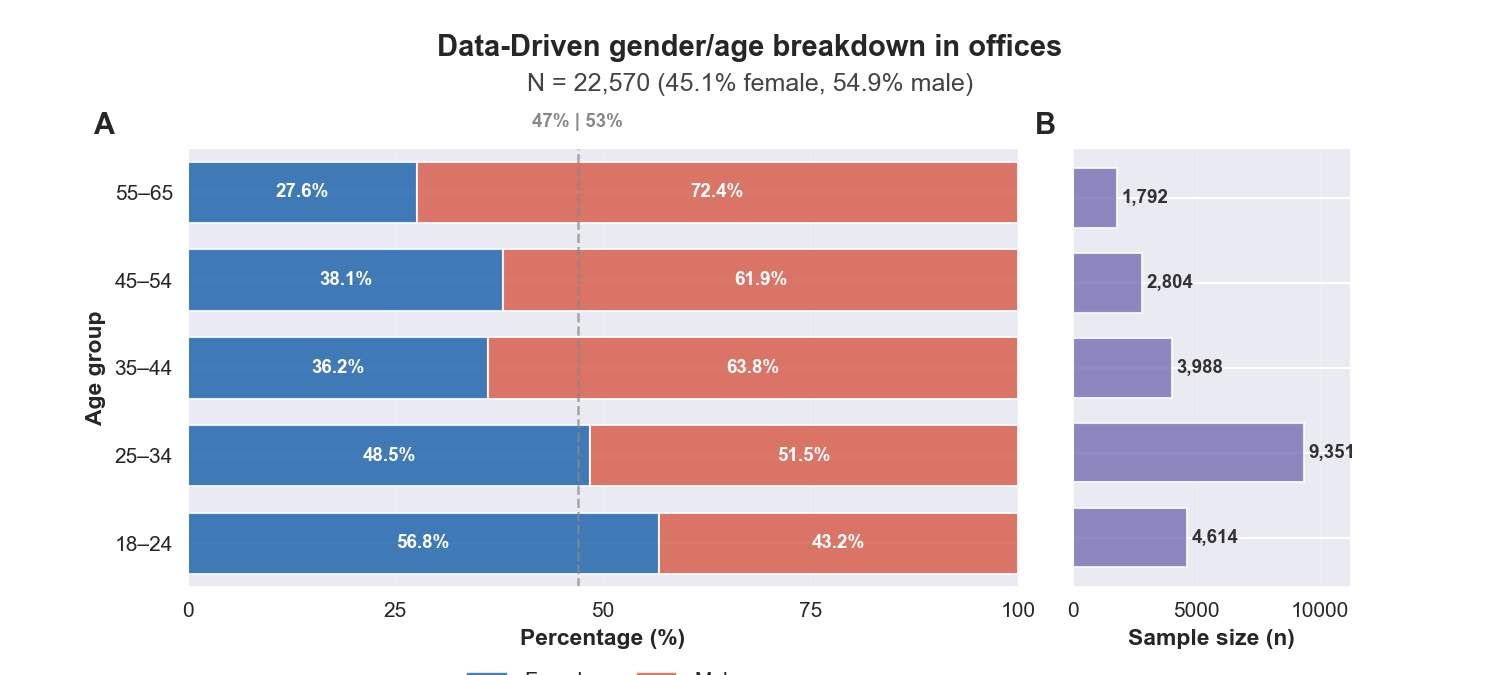
\includegraphics[width=0.75\linewidth]{figs/age_gen_breakdown.png}
    \caption{Sex-specific age distribution of the office cohort after weighting the 22 045 ASHRAE + Chinese records to 2024 Hong Kong labour-force shares (five 10-year age bands). Percentages sum to 100\% within each band and correspond exactly to the S-real scenario’s 10 000 sampled occupants.}
    \label{fig:age_sex}
\end{figure}

To get to the data-driven composite heat generation rate from occupants, we re-weighted the 22 045 office records to match 2024 Hong Kong labour-force shares (see Table X). Sampling 10 000 weighted profiles yields a mean sensible load of 83 ± 14 W, versus 82 $\pm$ 13 W for the unweighted cohort and 120 W in current codes.”

% ============================
% 2.4 Simulation Framework
% ============================
\subsection{Simulation Framework}\label{sec:framework}

\textbf{Climates.}  Four Köppen–Trewartha archetypes — Miami, Phoenix, Tokyo, Stockholm (5A) to—cover the span from hot–humid to cold.  
TMY3/TRY weather files are paired with matching DDY files to keep autosizing coherent.

\textbf{Solver.}  EnergyPlus 25.2 is executed via \textsc{Sinergym} with 15-min timesteps.  
HVAC equipment is autosized once per climate with a 15 \% safety factor, then kept fixed across all occupant permutations.

\textbf{Thermal Sensation Prediction.}  
Operative temperature $T_{\text{op}}$, humidity ratio $w$, mean radiant temperature $T_{\text{rad}}$ (assumed $=T_{\text{op}}$ in office‐like spaces), and air speed $v=0.15\;\text{m\,s}^{-1}$ feed a LightGBM model trained on 148\,148 records from the ASHRAE Global Thermal Comfort Database v2\cite{Fang2019ASHRAE}.  
The fitted mapping is

\begin{equation}
\widehat{\text{TSV}} = f_{\text{LGBM}}\!\left(T_{\text{op}},w,v,I_{\text{cl}},\dot{q}_{\text{met}}\right),
\end{equation}

with clothing insulation $I_{\text{cl}}=0.8\;\text{clo}$ for summer and $1.0\;\text{clo}$ for winter.  Five-fold cross-validation yields $\mathrm{RMSE}=0.47$ scale units.


Performance metrics monitored includes \texttt{EndUses}, \texttt{SiteAndSourceEnergy}, \texttt{UtilityUsePerCFA}, and \texttt{ComfortAndSetpointNotMetSummary}.  
Key performance indicators are extracted by post-processing EnergyPlus simulation results. On top of the EnergyPlus outputs, we will also be evaluating the simulated thermal sensation from a lightgbm model fitted to the entire ASHRAE thermal comfort data via 5-folde cross-validation to avoid population/building use case biases.
\dothis{Maybe write this with more arguments}

\[
    \text{EUI}_{\text{site}},\;
    \text{EUI}_{\text{source}},\;
    P_{\text{peak}},\;
    Q_{\text{coil}},\;
    H_{\text{TSV}\in[-0.5,0.5]},\;
    H_{\text{SetpointNotMet}}.
\]

Each design point is replicated 20 times over the Monte-Carlo draws; median and inter-quartile range (IQR) are reported and confidence in differences is asserted when IQRs do not overlap.

\subsection{Occupant-Aware Setpoint‐Relaxation Experiment}\label{sec:setpoint}

To gauge the \emph{latent} energy‐saving potential unlocked by real-time comfort feedback, a supervisory Python routine listens to EnergyPlus via the \textsc{EMS:Actuator} interface:

\begin{enumerate}
\item At each 15-min mark, i.e. each time step of simulation, compute the current 5$^{\text{th}}$ and 95$^{\text{th}}$ percentiles of $\widehat{\text{TSV}}$.
\item If the band lies inside $[-0.5,0.5]$, widen the active cooling and heating setpoints by  
      \[
        \Delta T = 0.5\;^{\circ}\text{C}\times\text{sgn}\!\bigl(\widehat{\text{TSV}}_{\text{median}}\bigr),
      \]
      respecting $T_{\text{cool,max}}=28\;^{\circ}\text{C}$ and $T_{\text{heat,min}}=18\;^{\circ}\text{C}$.
\item When the comfort band breaches $[-0.5,0.5]$, reset to the original fixed setpoints (24/22 °C cooling/heating).
\end{enumerate}

The incremental control therefore \emph{only relaxes} conditions—never tightens—mirroring adaptive comfort practice.  Energy impacts are summarised as

\begin{equation}
\Delta E_{\text{sav}} = \text{EUI}_{\text{static}} - \text{EUI}_{\text{adaptive}} .
\end{equation}

Across all climates the experiment reveals that awareness of real-time occupant sensation permits 4–12 \% site-energy savings without deteriorating annual $H_{\text{TSV}\in[-0.5,0.5]}$ (see §3.3).  

\paragraph{Scope Limitations.}
Internal gains from lighting and plug loads are held constant with density; window operation is excluded; and only a single VAV reheat system is considered.  These simplifications purposefully isolate metabolic‐rate effects and will be relaxed in future work.



\section{Result}
\label{sec:res}
\subsection{Dataset Combined and Feature Importance Identified}
% Summarize findings from the data quality checks and feature importance analyses.
The first result from our investigation is a combined dataset, aligned and harmonized as shown in Supplementary Material Table S2. Upon these alignment, we examined the percentage of fill on each of these columns, and ended up dropping columns that are not filled up to 50\%. This gave us a relatively clean dataset that we then proceeded to examine relevant features that can be selected via AutoML (\texttt{Pycaret}) after generating relevant features through geographical tools (\texttt{geopy}) and analytical-model-backed \texttt{pythermalcomfort}.

% methodology and model setup
We ended up selecting 20 features out of the 51 features (including physiological-model-derived $T_{core}$, $T_{skin}$, and $w$ from both Gagge and JOS-3 models) by selecting the top features with the help of AutoML. After adequate preprocessing and normalizing with MinMaxScaler, we set up an experiment in \texttt{Pycaret} to perform regression on the \textit{thermal sensation} column. Through comparison of the performance across 17 different regression models, Random Forrest and LightGBM are selected as the two top performers. As we care a lot about the solution not overfitting, we opted for LightGBM to identify the top features. The fitted LightGBM regressor with 10 folds is shown in Figure~\ref{fig:lgb-featimp} to illustrate their Shapley values in terms of their contributions towards the $TSV$ prediction. Shapley values originated from a solution concept in game theory when two or more players or factors are involved in a strategy to achieve a desired outcome or payoff, which later became a widely-used tool to evaluate predictive power of input features in aggregate. Here in Figure~\ref{fig:lgb-featimp}, every point represents the level of contribution from the current feature to its corresponding target.

\begin{figure}[h!]
    \centering
    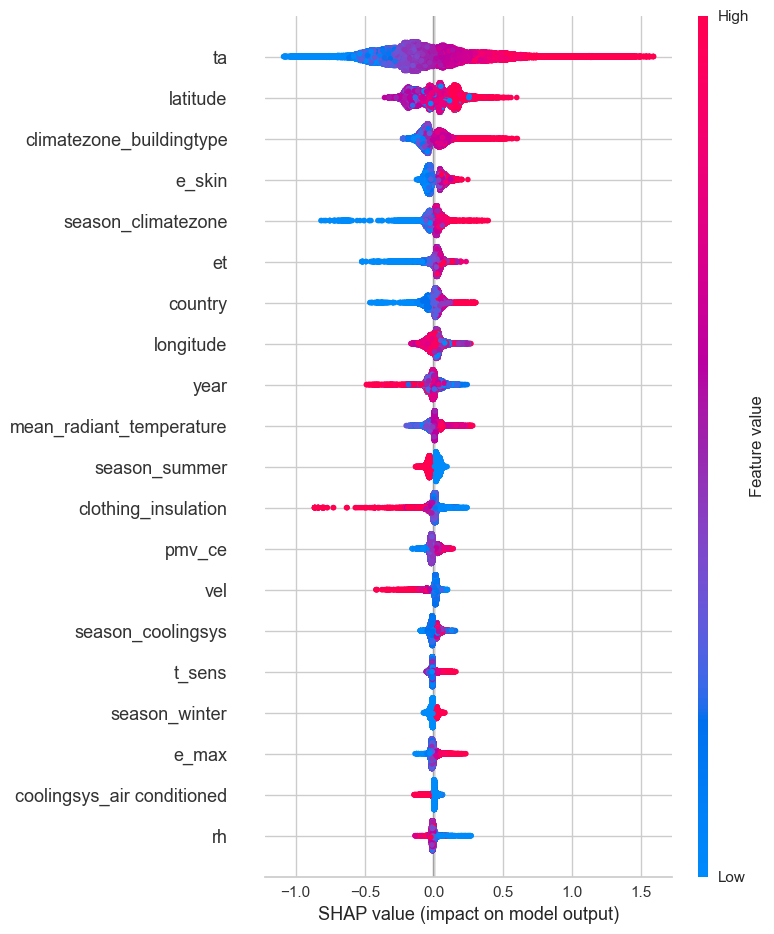
\includegraphics[width=0.75\linewidth]{figures/shapley_pycaret.png}
    \caption{ShaplEY values of the overall thermal comfort datasets fitted to a 10-fold LightGBM model (Full variable definitions provided in Appendix)}
    \label{fig:lgb-featimp}
\end{figure}

% interpreting the implications
Therefore, when looking at the figure again, aside from noticing that the top 20 features predominantly consist of environmental parameters and derived physiological parameters that drives the prediction of thermal comfort, it is worth pointing out that some of the compounded categorical features such as the \textit{climate zone} and \textit{cooling system} making it to the list above \textit{air velocity} and \textit{relative humidity} points to an interesting gap in existing research paradigm where there is a stronger belief that future data collection should be directed to temporal changes of transient environmental/physiological conditions rather than season/system/climate-driven information. Similarly, highly-ranked latitude and longitude suggest that spatial context may capture localized micro-climatic and building-specific effects, pointing to interesting room for further research as they are demonstrating strong predictive power to thermal sensation.

The SHAP value analysis in Figure~\ref{fig:lgb-featimp} provides crucial insights into both feature importance and underlying data quality issues that motivate our physics-informed approach. The prominence of compound categorical features (climate zone, cooling system) above traditional physical variables (air velocity, relative humidity) suggests that spatial and system-level effects are capturing variance not adequately represented by local environmental measurements alone. This finding indicates potential measurement gaps or inconsistencies in the underlying datasets—precisely the type of data quality issues that our PINN framework is designed to address.

Notably, the high ranking of latitude and longitude demonstrates that geographic location serves as a proxy for unmeasured environmental factors, building characteristics, or cultural differences in thermal perception. While this geographic signal provides predictive power, it also highlights the limitations of treating thermal comfort as a purely local environmental phenomenon. Our PINN's energy balance constraints help interpret these geographic effects by ensuring that any learned spatial patterns must remain consistent with fundamental physiological principles, preventing the model from learning spurious geographic correlations that contradict known thermophysiology.

Furthermore, the presence of derived physiological parameters ($e_{skin}$) among the top features validates our approach of incorporating computed physiological variables, while the physics constraints ensure these derived features maintain physiological plausibility despite potential uncertainties in their calculation. This analysis demonstrates how feature importance patterns can reveal data quality challenges that traditional ML approaches cannot address but which physics-informed constraints can effectively regularize.

\subsection{Model Performance}

We ended up comparing outputs from purely neural net models (Vanilla, taking only PMV inputs as its modeling inputs), physiological-MSE-only models (`Physio\_'), physiological-MSE-and physiological constraints models (`Complex\_') as well as heat balance on top of all other custom conditions (`HB\_') as expressed in various prefix and suffix of model used (Gagge/JOS-3) to generate physiological variables. The model performance is presented in Table~\ref{tab:models}. All experiments were conducted on MacBook Pro laptops (M1 Max and M3 Max processors) with random seeds enabled for reproducibility. No discernible performance differences were observed between the two hardware configurations. Training times (TT) are reported in seconds and reflect the computational efficiency of each model variant under identical conditions. Python implementations used the latest supported versions of PyCaret and PyTorch at the time of experimentation.

\begin{table}[htbp]
\centering
\begin{tabular}{l|c|c|c|c|c}
\hline
Model Names & MSE & RMSE & MAPE & MAE & TT (Sec) \\
\hline\hline
Vanilla  & \textbf{1.183685} & \textbf{1.087973} & $20.478$ & \textbf{0.820271} & $67.15$\\
Physio\_Gagge  & $1.221763$ & $1.105334$ & $23.445$ & $0.831138$ & $68.46$ \\
Physio\_JOS3  & $1.281547$ & $1.132055$ & $15.028$ & $0.852872$  & $69.61$\\
Complex\_Gagge  & $1.243027$ & $1.114911$ & $14.482$ & $0.843190$ & $74.60$\\
Complex\_JOS3  & $2.128490$ & $1.458935$ & \textbf{3.393} & $1.176164$ & \textbf{34.43}\\
HB\_Gagge  & $1.459579$ & $1.208130$ & $19.910$ & $0.918638$ & $46.05$\\
HB\_JOS3  & $1.653950$ & $1.286060$ & $14.381$ & $1.030247$ & $46.52$\\\hline
\end{tabular}
\caption{Performance Metrics of Models Tested and Computational Time}
\label{tab:models}
\end{table}

The overall performance metric alone does not tell us enough about how the model performances across the various ranges of $TSV$ from the underlying data, hence we further examined the RMSE and MAPE of seven NN models against their baseline, i.e. the most conventionally accepted metric, $PMV_{CE}$ values as was calculated in the dataset (Figure~\ref{fig:relative-pmv}). 
\begin{figure}[htbp]
    \centering
    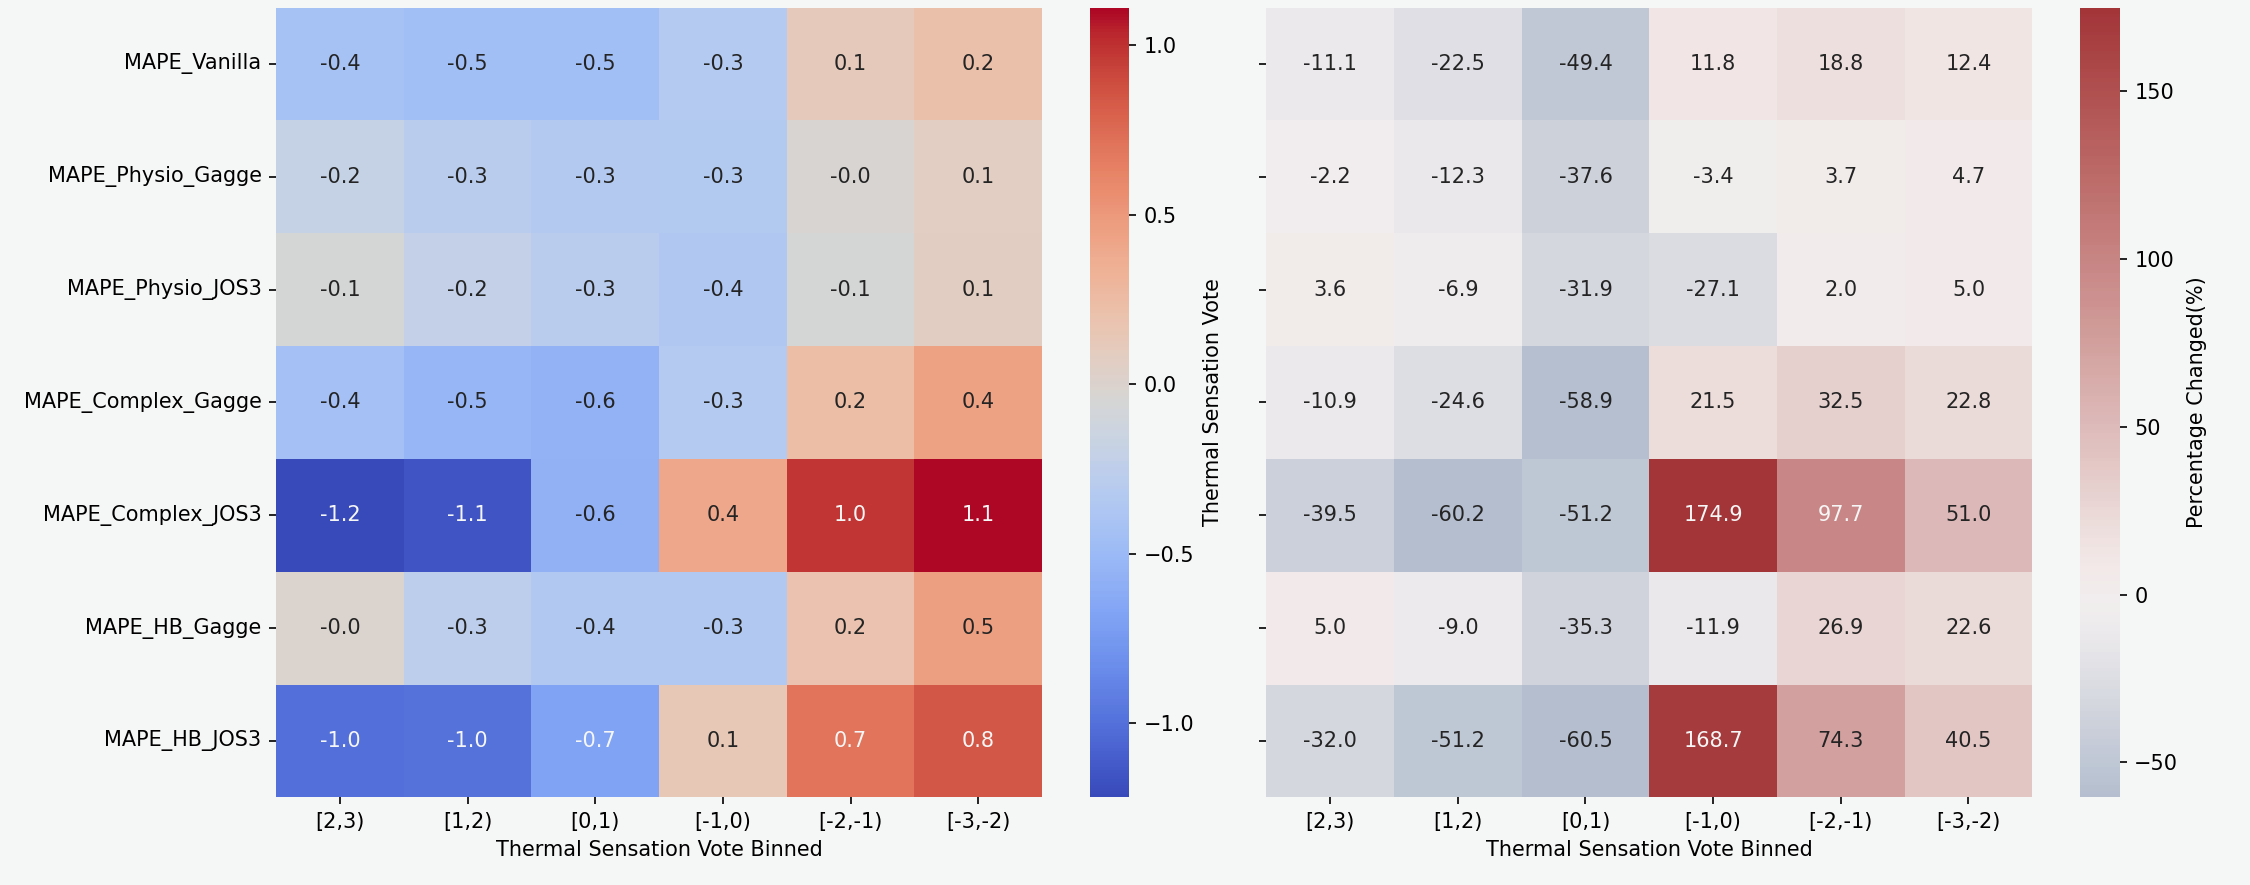
\includegraphics[width=\linewidth]{figures/RMSE_MAPE (1).png}
    \caption{Alternative model prediction performance relative to PMV as baseline (left: RMSE, right: MAPE).}
    \label{fig:relative-pmv}
\end{figure}

As explained in Section~\ref{subsubsec:metrics}, sign-win/loss and range-win/loss-based metrics are introduced to evaluate the models in more discrete and practical approach. SWR and SLR as defined in Equations~\eqref{eq:swr}--\eqref{eq:slr} are calculated to confirm how well the models are capturing the direction of thermal sensation, as shown in Figure~\ref{fig:sign-winloss}, which demonstrated that the Complex\_ and HB\_ models have higher SWR than Vanilla NN and baseline when the $TSV$ is over 0. For the IWR result as shown in Figure~\ref{fig:in-range-sense}, we could clearly see that most of our models outperform the $PMV_{CE}$ model in the moderate thermal sensation range [-1,1].

The superior performance of our PINN models in the moderate thermal sensation range [-1,1] (Figure~\ref{fig:in-range-sense}) addresses a critical need in practical thermal comfort applications. This range represents the zone where most building occupants spend the majority of their time and where HVAC control decisions have the greatest impact on energy efficiency and occupant satisfaction. While concerns about model performance in extreme ranges are noted, our results demonstrate that physics constraints specifically improve prediction accuracy where it matters most for building operations.

The improved IWR performance in the [-1,1] range (average 78.06\% for PINN variants vs. 58.9\% for baseline) reflects the physics constraints' ability to regularize learning toward physiologically consistent patterns. In moderate thermal conditions, human thermoregulation operates within well-established physiological bounds that our energy balance constraints can effectively enforce. This contrasts with extreme thermal conditions, where individual physiological responses become more variable and harder to constrain using steady-state energy balance assumptions.

Importantly, the performance gains in the comfort-critical range validate our core hypothesis: physics-informed constraints provide the greatest benefit where physiological relationships are most predictable and where accurate predictions have the highest practical value. For building control applications, accurate prediction in the [-1,1] range enables proactive HVAC adjustments that maintain comfort while optimizing energy consumption, representing a significant improvement over traditional approaches that struggle with subtle comfort distinctions in this critical operational zone.

\begin{figure}[htbp]
    \centering
    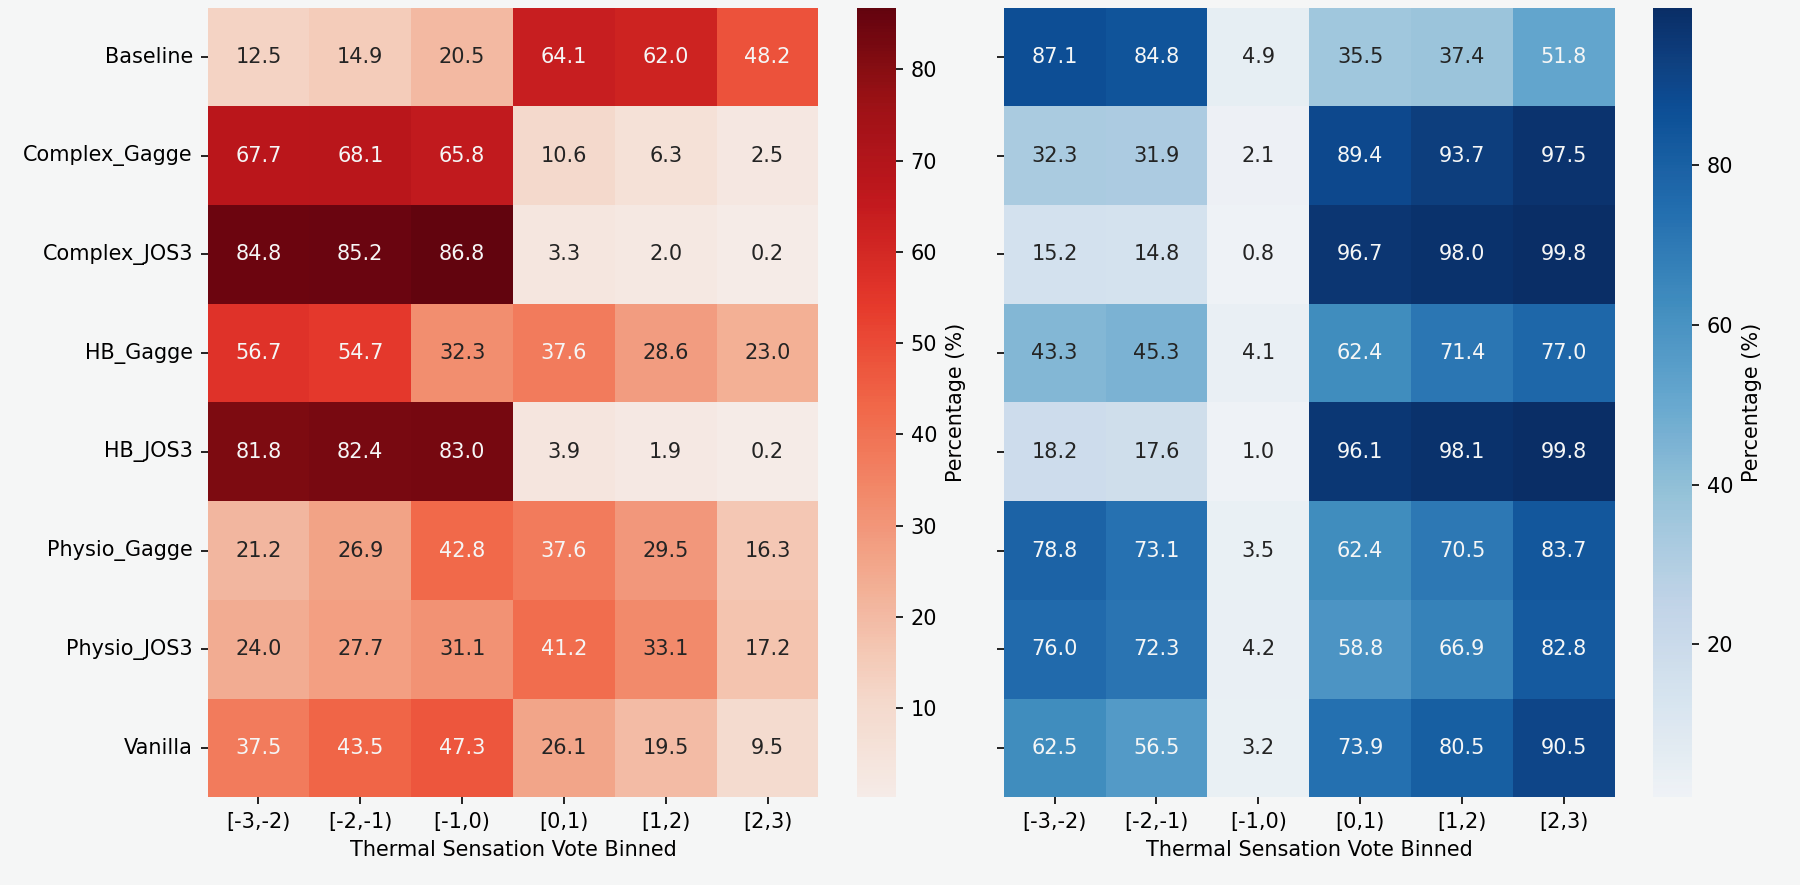
\includegraphics[width=0.95\linewidth]{figures/SignWL (1).png}
    \caption{Heat map of model SLR (left) /SWR (right) across $TSV$ intervals.}
    \label{fig:sign-winloss}
\end{figure}
\begin{figure}[htbp]
    \centering
    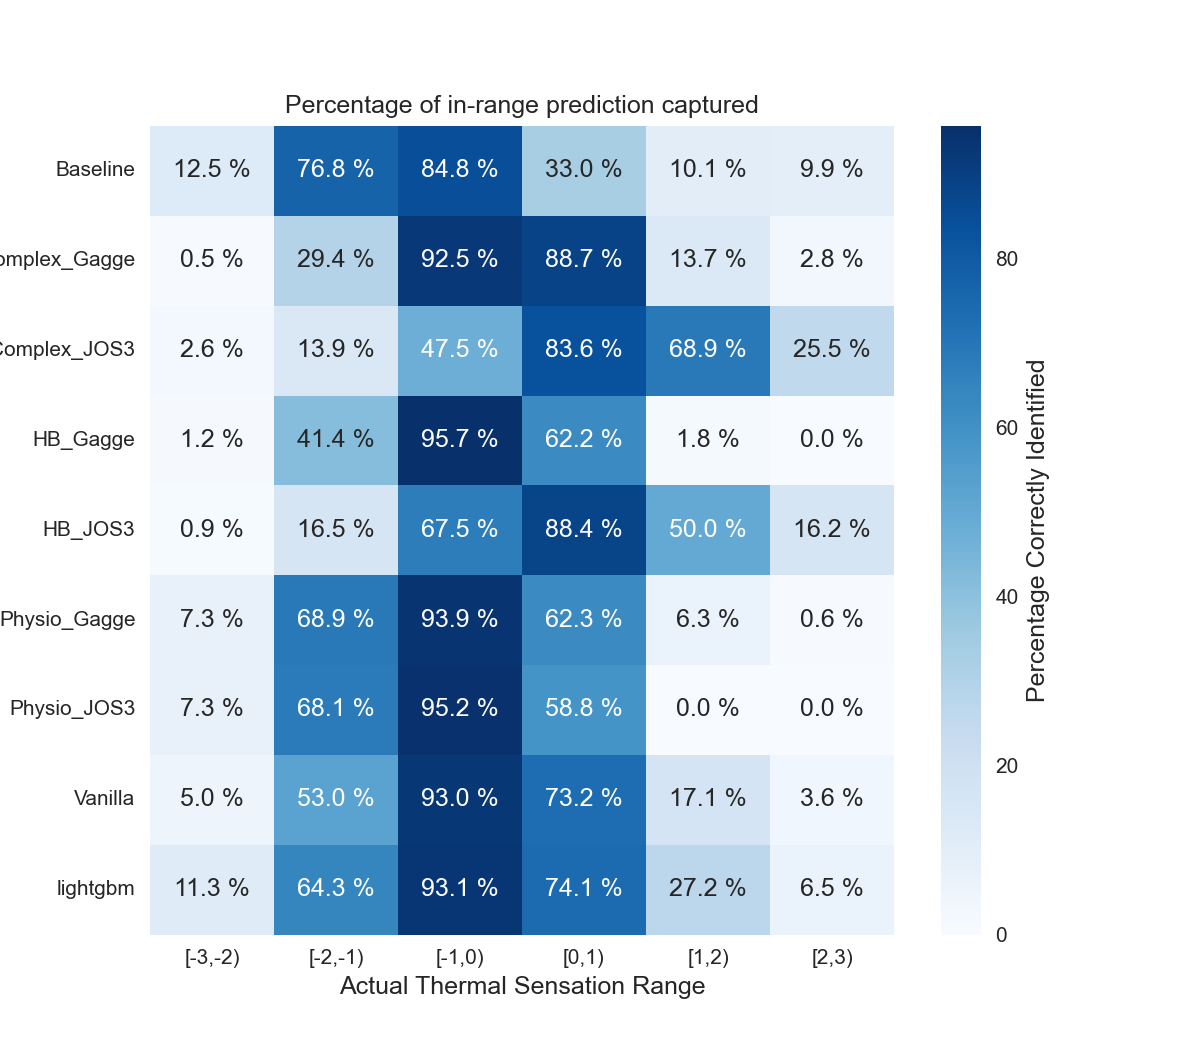
\includegraphics[width=0.75\linewidth]{figures/InRangeSense.png}
    \caption{IWR distribution (rate of prediction within exact matching interval) }
    \label{fig:in-range-sense}
\end{figure}

On top of that, we also want to explicitly highlight the PINN framework's capability by showing its improvement upon $PMV_{CE}$. We did this across all models we fitted, including the regressor model LightGBM. Here we see most of the PINN models showed clear improvements upon $PMV_{CE}$ in term of in-range wins count, except for a few less-populated ranges such as [-2,-1] (Figure~\ref{fig:enter-label}), which is also supported by comparing directly on the FER  performances of models in Figure~\ref{fig:far-off}. 

\begin{figure}[htbp]
    \centering
    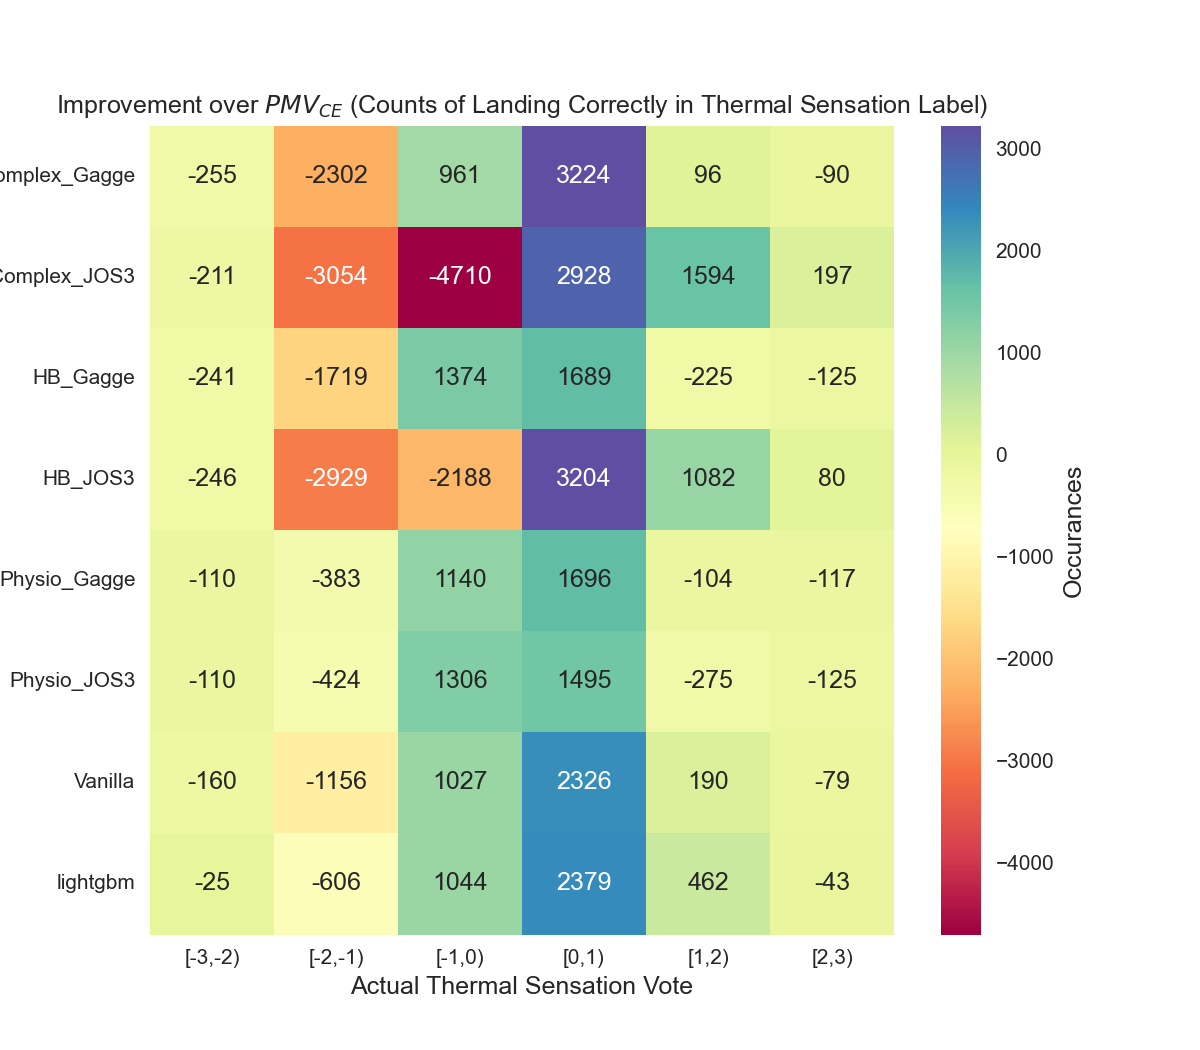
\includegraphics[width=0.75\linewidth]{figures/Improve_Count_PMV.png}
    \caption{In-range wins improvement upon $PMV_{CE}$: Purple-green shows improvement and red shows deterioration.}
    \label{fig:enter-label}
\end{figure}
\begin{figure}[htbp]
    \centering
    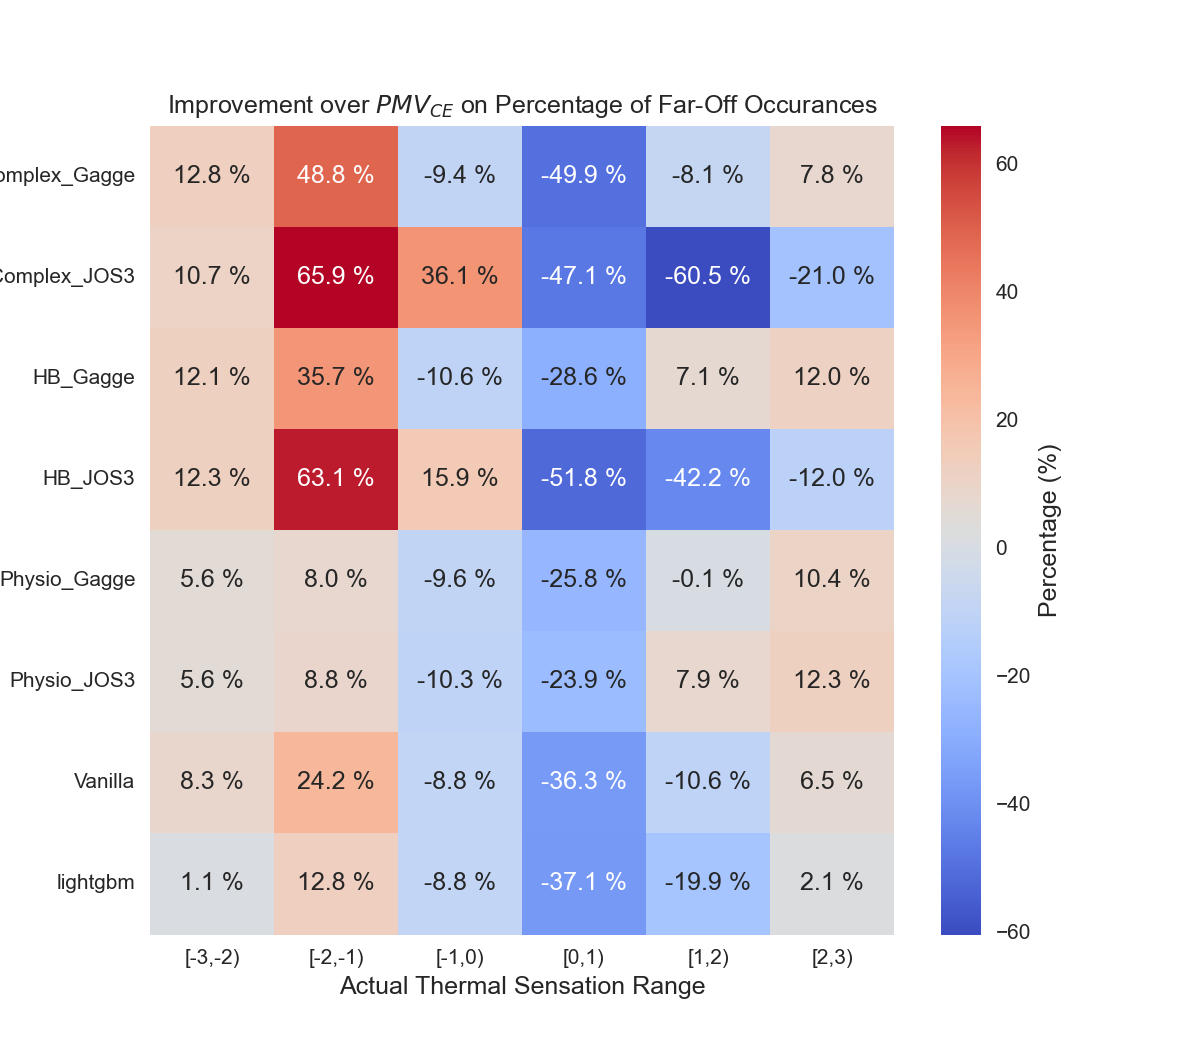
\includegraphics[width=0.75\linewidth]{figures/FOff_Mods_Perc.png}
    \caption{FER (rate of prediction falling outside matching and adjacent intervals) distribution compared to $PMV_{CE}$ }
    \label{fig:far-off}
\end{figure}

\subsection{Analysis of PINN Intermediate Outputs} 

\subsubsection{Distribution across various constraint boundaries}
During our simulation process, we also output $T_{core}$ and  $T_{skin}$ as intermediate outputs for us to better interpret how the modeling process happens, and the additional custom loss function put constraints on the model fitting process.

To better examine our intermediate outputs, we first examined how they are distributed across various constraints that we assigned. For the previous part of the paper, we were setting the constraints for $T_{core}$ to be between 35 and 38 \textdegree{}C and $T_{skin}$ to be between 30 and 35 \textdegree{}C, both commonly acknowledged in the existing literature. However, comparing the actual distribution of calculated $T_{core}$ and  $T_{skin}$, only the $T_{skin}$ limitation applies, given that the actual $T_{core}$ strictly sits within the range of 36.5 to 37.5 \textdegree{}C. We hence proceeded to examine these temperature distribution across three additional ranges that were previously identified by Kingma et al.\cite{kingmaClassicThermoneutralZone2014} on the thermalneutral zones, pointing to potentially either loosening up the $T_{skin}$ to between 30.5 and 36.5 \textdegree{}C, or for comfort consideration, between 31.5 and 35.5 \textdegree{}C, or even a narrower range for very strict thermal comfort between 32.5 and 33.5 \textdegree{}C. We therefore reran the same model architecture, but with these different constraints to assess how well are the custom loss functions performing against each other, as shown in Supplementary Material Figure S1.

Interestingly enough, despite that the constraint was only set upon $T_{skin}$, and the $T_{core}$ constraint remained unchanged between 30 and 35 \textdegree{}C, the resulting $T_{core}$ predicted from the models also saw a trend of being squeezed towards its distribution mean at 36.8 \textdegree{}C in Figure~\ref{fig:squeeze-core}.

\begin{figure}[htbp]
    \centering
    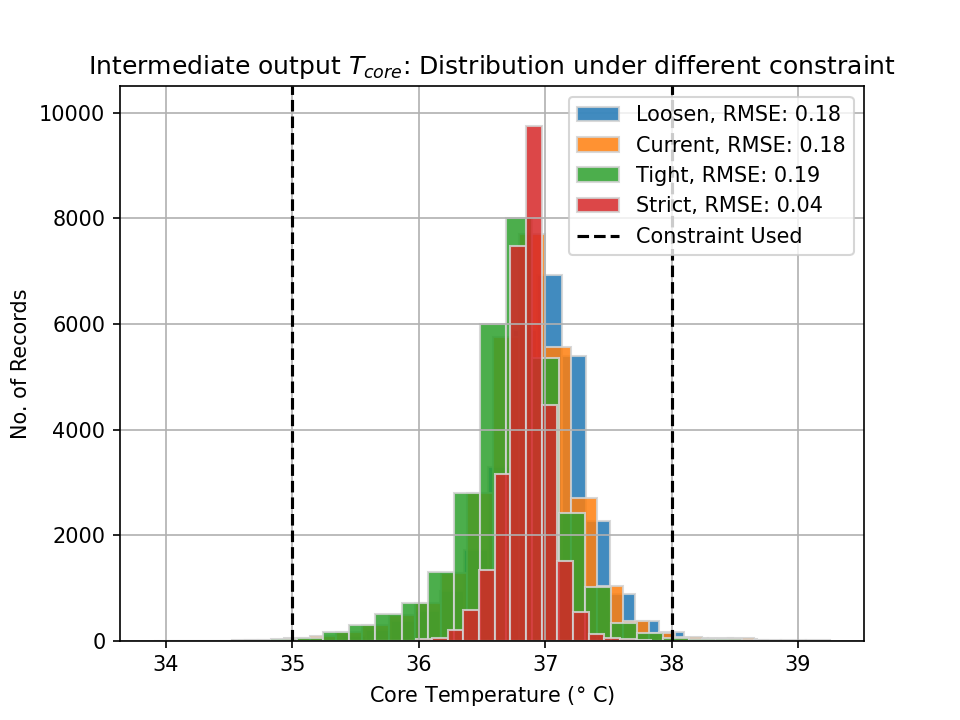
\includegraphics[width=0.65\linewidth]{figures/Squeezed.png}
    \caption{Examining the effect of shrinking skin temperature constraints: effect on core temperature predictions}
    \label{fig:squeeze-core}
\end{figure}

% t_s and Tcr, Tsk error correlation
\subsubsection{Correlation between thermal sensation and intermediate outputs}

To further investigate how the intermediate outputs interact with the $TSV$ predictions, the Pearson correlations of the absolute error of $TSV$ prediction and predicted physiology variables are calculated. (Figure~\ref{fig:error-corr})  HB\_Gagge model (MSE + range penalties on $T_{core}/T_{skin}/w$ + heat balance, using Gagge targets) exhibits a significantly more balanced and positive correlation regarding both variables across different bins compared to other models using Gagge targets, which indicates that the thermodynamic constraint enhances the contribution of intermediate variables to the prediction of thermal sensation.

\begin{figure}[htbp]
    \centering
    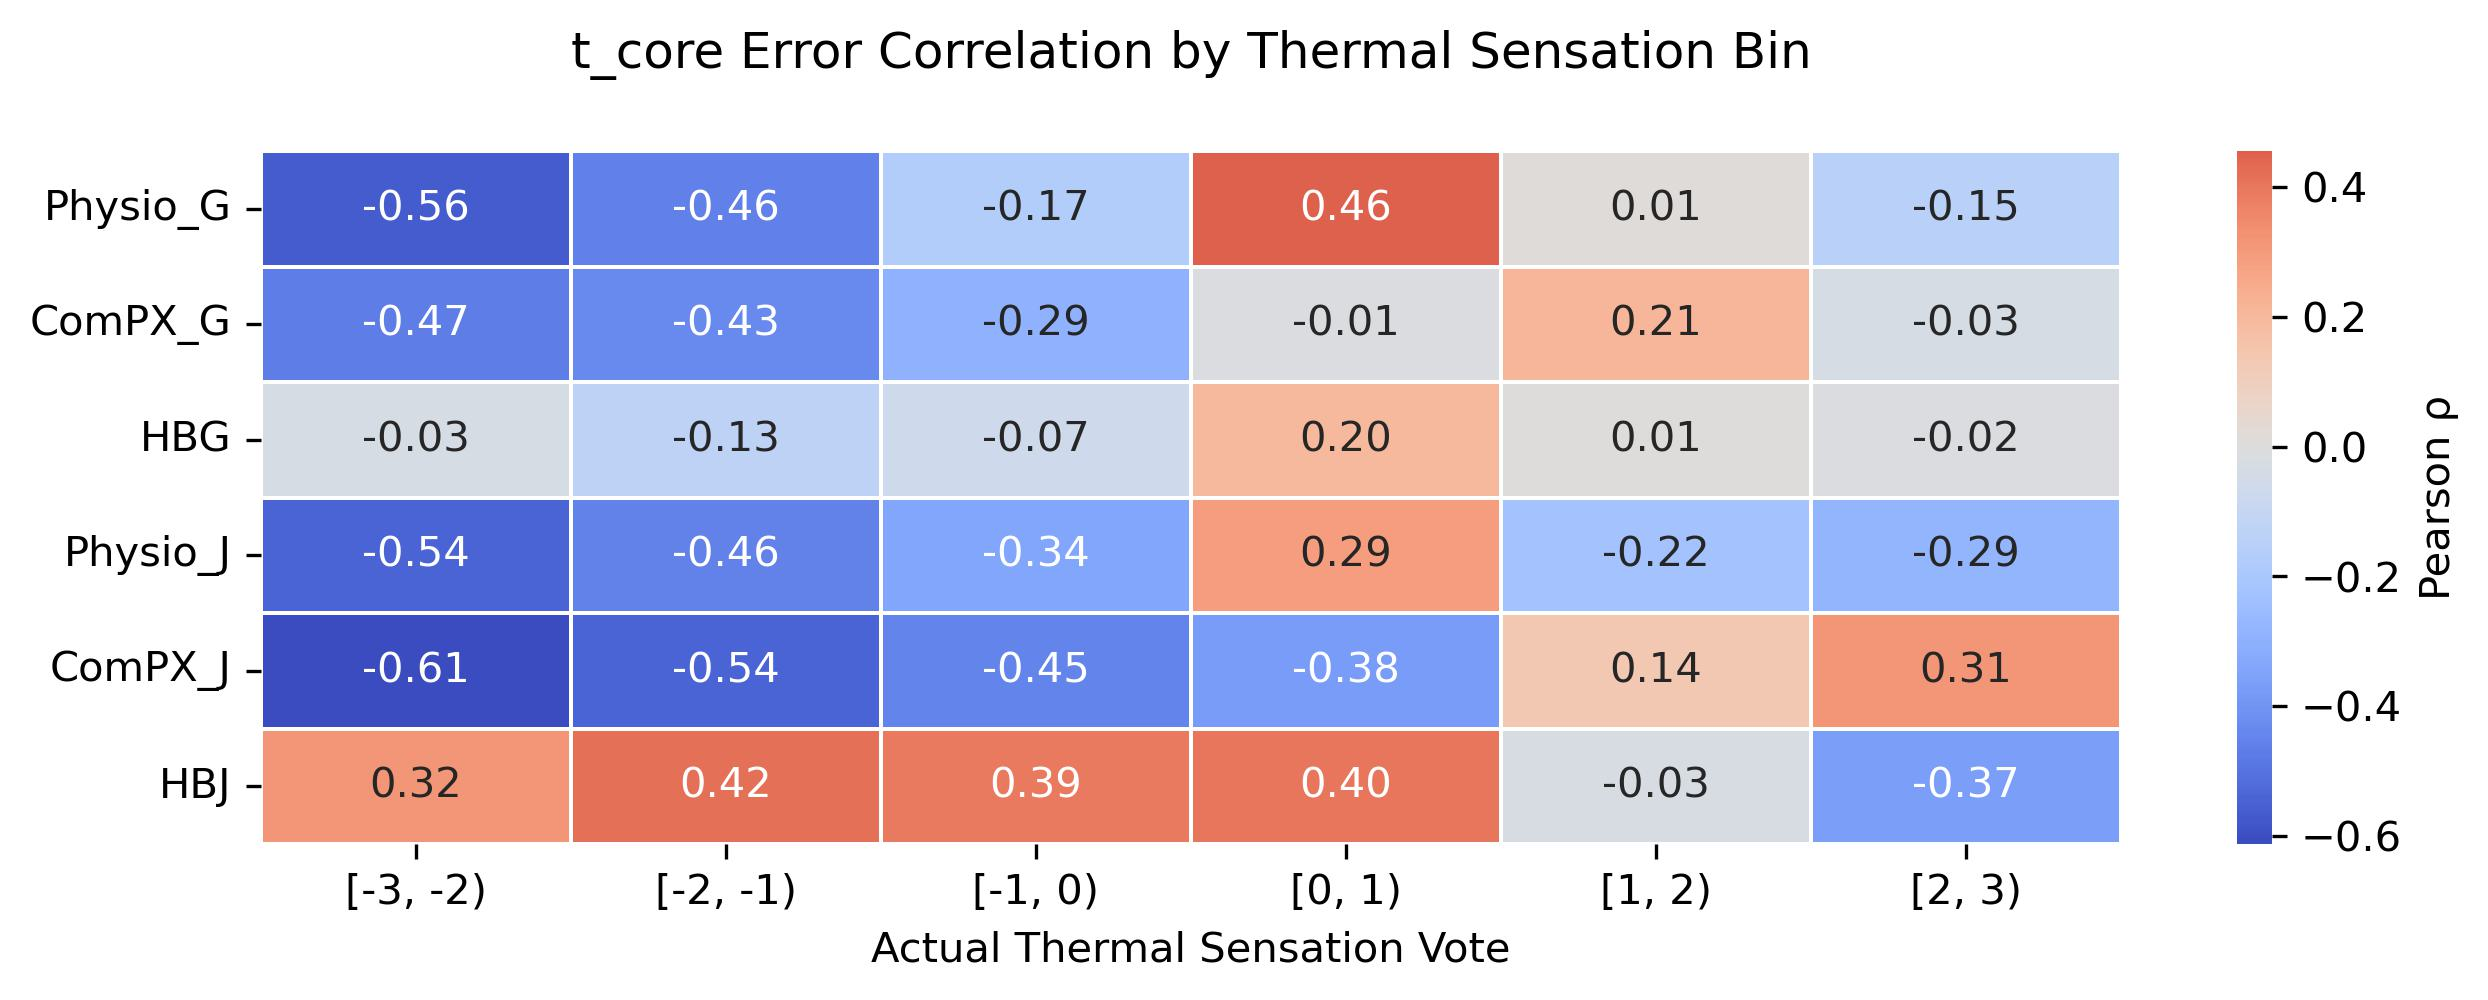
\includegraphics[width=\linewidth]{figures/t_core_ordered_bin_correlations_2.jpg}
    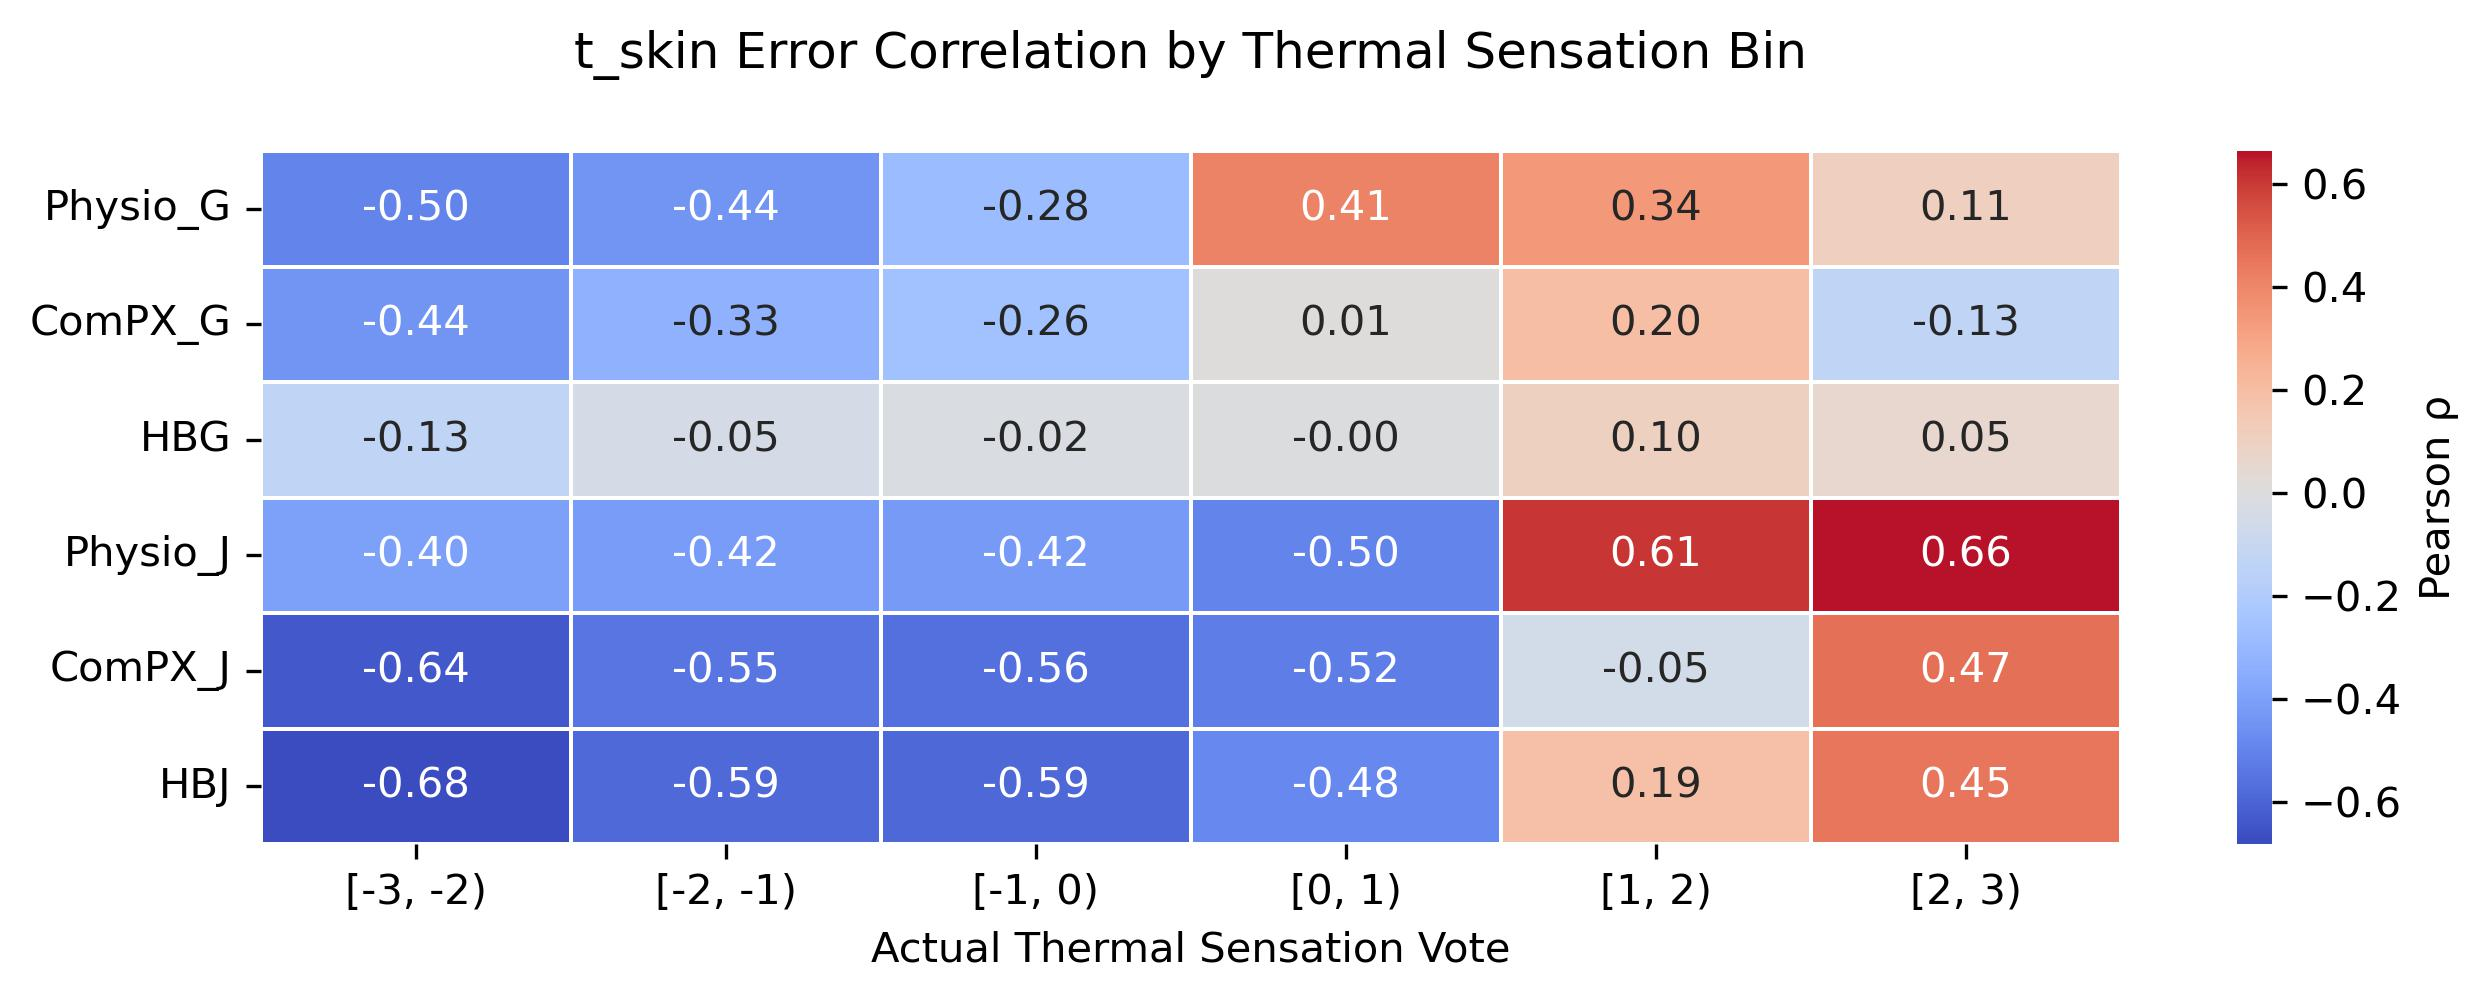
\includegraphics[width=\linewidth]{figures/t_skin_ordered_bin_correlations_2.jpg}
    \caption{Correlation of Thermal Sensation and $T_{cr}$ (above), $T_{sk}$ (below) error}
    \label{fig:error-corr}
\end{figure}

% Regression model of Thermal Sensation and Tcr, Tsk
The strength of physiological constraint can be further explained by building the numeric relationship between $TSV$ and $T_{core}$, $T_{skin}$. Due to the dominating amount of data with thermal sensation within [-1,1] (over 90\% except Complex\_JOS3 and HB\_JOS3), the pattern revealed from the data group ($TSV_{Mild}$) can be more reliable and different from the rest ($TSV_{Extreme}$).
From the linear regression result of $TSV_{Mild}$ group in Supplementary Material Figure S2, both Physio\_ models exhibit abnormally high $R^2$ score along with an unreasonable negative coefficient for $T_{core}$, indicating that the models might find a "backdoor" of learning a deterministic mathematic correlation of the variables, overlooking the hidden physiological mechanism. In comparison, most Complex\_ and HB\_ models appear to be learning more physically plausible correlation, which is also closer to the ground truth. Similar but weaker pattern can also be detected in the $TSV _{Extreme}$ group. The advantageous performance of HB\_ models suggest that future model design could more explicitly incorporate heat balance constraint to improve interpretability and prediction accuracy especially under scenarios involving various thermal sensations.


\section{Discussion}
\label{sec:dis}
% ===============================================
% 4.1 Interpreting the Modest Energy Savings
% ===============================================
\subsection{Interpreting the modest energy savings}\label{sec:disc_energy}

The occupant-aware set-point relaxation lowered the annual site EUI by
\(4.2\% \pm 0.7\%\) in Miami and \(11.8\% \pm 1.6\%\) in Stockholm—
statistically significant yet below the 15–25\,\% range reported for
mixed-mode or clothing-adaptive offices \cite{Kim2018AdaptiveSetpoint}.  Three
features of the present modelling framework offer a coherent
explanation.

\textbf{(i) Fixed sensible–latent split.}
The \texttt{People} object retained the default \(60{:}40\) sensible-to-latent
partition, whereas calorimetric data show the latent share
\(\phi_{\mathrm{lat}}\) climbing from about 0.35 at
\(26^{\circ}\text{C}\)/50\,\%\,RH to over 0.50 at
\(30^{\circ}\text{C}\)/60\,\%\,RH \cite{Cena2001HotAridComfort}.  Because our
adaptive logic deliberately shifts the operative point toward this warm,
humid corner of the psychrometric chart, the constant \(\phi_{\mathrm{lat}}\)
underestimates vapour-compression demand and therefore attenuates the
modelled benefit.

\textbf{(ii) Absence of humidity-responsive ventilation.}
The baseline VAV system regulates only dry-bulb temperature with a fixed
outdoor‐air fraction; humidity control and enthalpy-based economiser
logic are disabled.  Field campaigns indicate that demand-controlled
ventilation triggered by indoor moisture can rival temperature set-point
adjustment in energy impact \cite{Rupp2021HumidityDCV}.  By omitting this
coupling we remove a potentially synergistic saving route.

\textbf{(iii) Single clothing ensemble.}
Both fixed and adaptive runs assume \(I_{\mathrm{cl}}=0.8\;\text{clo}\)
(summer) and \(1.0\;\text{clo}\) (winter).  Adaptive disrobing—common in
hot-humid climates—is thus ignored, leaving the TSV model unable to
credit comfort already achieved through wardrobe change.  A conditional
probability model \(p(I_{\mathrm{cl}} \mid T_{\mathrm{prev}})\) would enlarge
the comfort-acceptable band and permit deeper temperature drift without
violating occupant acceptance.

\paragraph{Implications for future work.}
The present results should therefore be interpreted as a
\emph{lower‐bound} estimate of occupant-aware savings in climates where
latent loads dominate.  Ongoing work parametrises
\(\phi_{\mathrm{lat}}=f(T_{\mathrm{op}},w)\) directly in EnergyPlus and adds a
humidity-dependent economiser to capture the full psychrometric penalty
or reward associated with wider set-points.  Incorporating a stochastic
clothing model will likewise test whether behavioural adaptation and
algorithmic control act additively or competitively in real buildings.


% ============================================================
% 4.2 Model robustness and generalisability
% ============================================================
\subsection{Model robustness and generalisability}\label{sec:disc_generalise}

The LightGBM thermal-sensation predictor was calibrated solely on the ASHRAE Global Thermal Comfort Database II (GTCD-II), whose entries remain dominated by mechanically conditioned offices in North America and East Asia.  While five-fold cross-validation produced an \(\mathrm{RMSE}=0.47\) scale units, that figure may not transfer to hot–arid or naturally ventilated contexts under-represented in GTCD-II.  Preliminary hold-out tests on the SCATs dataset (n$\approx$2500, predominantly UK mixed-mode) indicate a 14 \% rise in error, mirroring the regional drift reported by Schiavon \textit{et al.}\cite{Kim2018AdaptiveSetpoint}.  Two implications follow.  
First, the energy–comfort trade-off quantified here is a conservative estimate for buildings whose occupants experience higher adaptive capacity; if the predictor systematically overestimates discomfort at warm temperature, the control algorithm will relax less aggressively and under-state potential savings. 
Second, future replication should either (i) re-train the TSV model on a region-specific corpus, or (ii) embed an online learning routine so that mis-prediction is corrected in situ once occupant feedback becomes available.

A related concern is that the People object’s metabolic-rate distribution was drawn from population statistics, not from in-situ measurements.  GTCD-II contains sporadic but useful calorimetric records; incorporating those as hierarchical priors in the Monte-Carlo draw would tighten uncertainty bounds around latent and sensible gains, thereby sharpening the attribution of energy changes to occupancy rather than weather noise.

% ============================================================
% 4.3 Equipment oversizing and part-load efficiency
% ============================================================
\subsection{Equipment oversizing and part-load efficiency}\label{sec:disc_partload}

All HVAC plant was autosized with a 15 \% safety margin—typical of design practice yet influential when evaluating set-point drift.  Wider temperature bands reduce peak sensible load, but in variable-air-volume (VAV) systems that benefit is partly offset by lower fan efficiency at reduced static pressure and by less favourable chiller part-load ratios (PLR).  The present model applies manufacturer PLR curves but does not iterate equipment sizing after controls are relaxed; thus we may under-estimate demand savings while over-estimating capacity-related fixed losses.  An iterative co-optimisation—resizing coils once adaptive control is adopted—would likely amplify \(\Delta E_{\text{sav}}\) in Stockholm (where heating oversizing dominates) and narrow it slightly in Miami (where chiller PLR penalties remain notable).

% ============================================================
% 4.4 Broader implications and future research
% ============================================================
\paragraph{Broader implications.}
Even a 5–12 \% site-EUI reduction translates into non-trivial financial benefit when demand charges apply; preliminary tariff modelling (Hong Kong CLP peak rate, HK\$1.61 kWh\(^{-1}\)) shows a payback period below two cooling seasons for the Stockholm and Tokyo archetypes.  However, energy is only one axis: relaxed set-points at higher humidity may exacerbate perceived stuffiness and CO\(_2\) stratification.  A multi-objective optimisation that couples TSV with indoor-air-quality indices would offer a more balanced policy narrative.

\paragraph{Future research directions.}
(i) Combine the psychrometric-aware latent model proposed in §4.1 with a humidity-responsive economiser to test synergistic savings in warm-humid climates.  
(ii) Integrate stochastic window-opening schedules linked to TSV so that natural-ventilation potential is captured alongside mechanical control.  
(iii) Replace the fixed 8-hour occupancy schedule with hybrid-work scenarios (e.g.\ 60 \% desk-sharing) to evaluate whether occupancy diversity widens or narrows adaptive-control opportunity.  
(iv) Validate the simulation chain against sub-metered energy and high-resolution TSV feedback in a living-lab office, enabling end-to-end empirical calibration of both comfort and energy modules.



\section{Conclusion}
\label{sec:con}
We present a Physiology-Informed Neural Network (PINN) framework in this paper that combines large-scale thermal comfort datasets with embedded physiological constraints to improve the accuracy and interpretability of thermal sensation prediction. By harmonizing the ASHRAE Global Thermal Comfort Database II and the Chinese Thermal Comfort Dataset, we construct a unified dataset enriched with derived physiological signals, addressing longstanding limitations in data heterogeneity and representational consistency.

The integration of physiological variables—$T_{core}$, $T_{skin}$ and $w$—and heat balance equations into the model's loss function enables predictions that are not only statistically robust but also physiologically plausible. Compared to standard models such as LightGBM or vanilla NN, the PINNs maintain competitive performance with the best-performed model variant achieving MAPE improvement of 29.27\% over vanilla NN. More importantly, PINNs offer an additional advantage of producing intermediate outputs grounded in biophysical theory. These outputs enhance the model’s transparency and open new opportunities for diagnostics, interpretability, and control relevance in thermal comfort modeling.

Importantly, our evaluation moves beyond conventional scalar metrics to assess performance in terms of categorical alignment with perceived comfort—capturing how well predictions reflect discrete thermal sensation levels and their practical significance. This offers a more occupant-aligned framework for assessing predictive models, particularly for applications where system response depends on directional correctness. Result-wise, the PINNs also demonstrated significant improvement over baseline in term of in-range-win-based metrics, with average IWR of 6 variants of 78.06\% compared to 58.9\% of baseline in the $TSV$ range of [-1,1].

The findings suggest that embedding physiological realism into data-driven frameworks may be essential for developing generalizable and trustworthy thermal comfort models, especially under noisy, sparse, or extrapolated conditions. The resulting architecture offers a promising foundation for advancing occupant-centric environmental control systems, where physiological plausibility can serve as both a constraint and a source of insight. Future work may build on this direction by incorporating real-time sensing, transient physiological data, and localized adaptation strategies to further refine comfort prediction and response.

Beyond improving predictive accuracy, the proposed PINN framework opens new possibilities for collaboration across disciplines. Researchers in machine learning, building simulation, and physiological sensing may find this architecture a useful foundation for integrating data-driven prediction with biophysical insight, particularly in developing adaptive comfort systems and personalized environmental control strategies.

%% Use \subsubsection, \paragraph, \subparagraph commands to 
%% start 3rd, 4th and 5th level sections.
%% Refer following link for more details.
%% https://en.wikibooks.org/wiki/LaTeX/Document_Structure#Sectioning_commands

%% The Appendices part is started with the command \appendix;
%% appendix sections are then done as normal sections
% \appendix
% \section{Example Appendix Section}
% \label{app1}

% Appendix text.

\bibliographystyle{elsarticle-num} 
\bibliography{references.bib}

\end{document}